%%%%%%%%%%%%%%%%%%%%%%%%%%%%%%%%%%%%%%%%%%%%%%%%%%%%%%%%%%%%%%%%%%%%%%%%%%%%%%%%
% Template for USENIX papers.
%
% History:
%
% - TEMPLATE for Usenix papers, specifically to meet requirements of
%   USENIX '05. originally a template for producing IEEE-format
%   articles using LaTeX. written by Matthew Ward, CS Department,
%   Worcester Polytechnic Institute. adapted by David Beazley for his
%   excellent SWIG paper in Proceedings, Tcl 96. turned into a
%   smartass generic template by De Clarke, with thanks to both the
%   above pioneers. Use at your own risk. Complaints to /dev/null.
%   Make it two column with no page numbering, default is 10 point.
%
% - Munged by Fred Douglis <douglis@research.att.com> 10/97 to
%   separate the .sty file from the LaTeX source template, so that
%   people can more easily include the .sty file into an existing
%   document. Also changed to more closely follow the style guidelines
%   as represented by the Word sample file.
%
% - Note that since 2010, USENIX does not require endnotes. If you
%   want foot of page notes, don't include the endnotes package in the
%   usepackage command, below.
% - This version uses the latex2e styles, not the very ancient 2.09
%   stuff.
%
% - Updated July 2018: Text block size changed from 6.5" to 7"
%
% - Updated Dec 2018 for ATC'19:
%
%   * Revised text to pass HotCRP's auto-formatting check, with
%     hotcrp.settings.submission_form.body_font_size=10pt, and
%     hotcrp.settings.submission_form.line_height=12pt
%
%   * Switched from \endnote-s to \footnote-s to match Usenix's policy.
%
%   * \section* => \begin{abstract} ... \end{abstract}
%
%   * Make template self-contained in terms of bibtex entires, to allow
%     this file to be compiled. (And changing refs style to 'plain'.)
%
%   * Make template self-contained in terms of figures, to
%     allow this file to be compiled. 
%
%   * Added packages for hyperref, embedding fonts, and improving
%     appearance.
%   
%   * Removed outdated text.
%
%%%%%%%%%%%%%%%%%%%%%%%%%%%%%%%%%%%%%%%%%%%%%%%%%%%%%%%%%%%%%%%%%%%%%%%%%%%%%%%%

\documentclass[letterpaper,twocolumn,10pt]{article}
\usepackage{usenix}


\section{Experiment Environment}
\label{sec:experiment_environment}

All the experiments were conducted on Linux server with 4 NVIDIA A100-SXM4-80GB GPUs. Its operating system is 20.04.5 LTS (Focal Fossa). We implemented our proposed model CORRECT using Python 3.9 as programming language and PyTorch 1.14.0 as deep learning library. Other frameworks include numpy 1.22.2, sklearn 0.24.2, and transformers 4.43.3.

\newcommand{\sysname}{{XPUT\textsc{imer}}}
\newcommand{\groupname}{{Ant Group}}
% \newcommand{\sysname}{{XPUT\textsc{imer}}}



% \newcommand{\sysname}{{R\textsc{adar}}}
%\newcommand{\cell}{{\emph{Cell}}}
%\newcommand{\peaktpt}{{1.49}}
%\newcommand{\queuet}{{71.0\%}}
%\newcommand{\jct}{{48.9\%}}

% to be able to draw some self-contained figs
% \usepackage{tikz}
% \usepackage{amsmath}

% inlined bib file
% \usepackage{filecontents}

%-------------------------------------------------------------------------------
% \begin{filecontents}{\jobname.bib}
% %-------------------------------------------------------------------------------
% @Book{arpachiDusseau18:osbook,
%   author =       {Arpaci-Dusseau, Remzi H. and Arpaci-Dusseau Andrea C.},
%   title =        {Operating Systems: Three Easy Pieces},
%   publisher =    {Arpaci-Dusseau Books, LLC},
%   year =         2015,
%   edition =      {1.00},
%   note =         {\url{http://pages.cs.wisc.edu/~remzi/OSTEP/}}
% }
% @InProceedings{waldspurger02,
%   author =       {Waldspurger, Carl A.},
%   title =        {Memory resource management in {VMware ESX} server},
%   booktitle =    {USENIX Symposium on Operating System Design and
%                   Implementation (OSDI)},
%   year =         2002,
%   pages =        {181--194},
%   note =         {\url{https://www.usenix.org/legacy/event/osdi02/tech/waldspurger/waldspurger.pdf}}}
% \end{filecontents}

%-------------------------------------------------------------------------------
\begin{document}
%-------------------------------------------------------------------------------

%don't want date printed
\date{}

% make title bold and 14 pt font (Latex default is non-bold, 16 pt)
\title{\Large \bf \sysname{}: Anomaly Diagnostics for Divergent LLM Training in \\ GPU Clusters of Thousand-Plus Scale}

%for single author (just remove % characters)
\author{
{\rm Weihao Cui$^{1}$\thanks{Weihao Cui and Ji Zhang contributed equally to this work.}, Ji Zhang$^{2}$\footnotemark[1], Han Zhao$^{1}$, Chao Liu$^{2}$, Wenhao Zhang$^{1}$, Jian Sha$^{2}$\thanks{Jian Sha and Quan Chen are the corresponding authors}}\\ 
{\rm Quan Chen$^{1}$\footnotemark[2], Bingsheng He$^{3}$, Minyi Guo$^{1}$}\\
$^{1}$Shanghai Jiao Tong University,$^{2}$Ant Group,$^{3}$National University of Singapore
} % end author

\maketitle

%-------------------------------------------------------------------------------
\begin{abstract}
%-------------------------------------------------------------------------------
The rapid proliferation of large language models has driven the need for efficient GPU training clusters. However, ensuring high-performance training in these clusters is challenging due to the complexity of software-hardware interactions and the frequent occurrence of training anomalies. Since existing diagnostic tools are narrowly tailored to specific issues, there are gaps in their ability to address anomalies spanning the entire training stack. In response, we introduce \sysname{}, a real-time diagnostic framework designed for distributed LLM training at scale. \sysname{} first integrates a lightweight tracing daemon to monitor key code segments with minimal overhead. Additionally, it features a diagnostic engine that employs novel intra-kernel tracing and holistic aggregated metrics to efficiently identify and resolve anomalies. Deployment of \sysname{} across 6,000 GPUs over eight months demonstrated significant improvements across the training stack, validating its effectiveness in real-world scenarios.
\end{abstract}

\section{Introduction}
\label{sec:introduction}
The business processes of organizations are experiencing ever-increasing complexity due to the large amount of data, high number of users, and high-tech devices involved \cite{martin2021pmopportunitieschallenges, beerepoot2023biggestbpmproblems}. This complexity may cause business processes to deviate from normal control flow due to unforeseen and disruptive anomalies \cite{adams2023proceddsriftdetection}. These control-flow anomalies manifest as unknown, skipped, and wrongly-ordered activities in the traces of event logs monitored from the execution of business processes \cite{ko2023adsystematicreview}. For the sake of clarity, let us consider an illustrative example of such anomalies. Figure \ref{FP_ANOMALIES} shows a so-called event log footprint, which captures the control flow relations of four activities of a hypothetical event log. In particular, this footprint captures the control-flow relations between activities \texttt{a}, \texttt{b}, \texttt{c} and \texttt{d}. These are the causal ($\rightarrow$) relation, concurrent ($\parallel$) relation, and other ($\#$) relations such as exclusivity or non-local dependency \cite{aalst2022pmhandbook}. In addition, on the right are six traces, of which five exhibit skipped, wrongly-ordered and unknown control-flow anomalies. For example, $\langle$\texttt{a b d}$\rangle$ has a skipped activity, which is \texttt{c}. Because of this skipped activity, the control-flow relation \texttt{b}$\,\#\,$\texttt{d} is violated, since \texttt{d} directly follows \texttt{b} in the anomalous trace.
\begin{figure}[!t]
\centering
\includegraphics[width=0.9\columnwidth]{images/FP_ANOMALIES.png}
\caption{An example event log footprint with six traces, of which five exhibit control-flow anomalies.}
\label{FP_ANOMALIES}
\end{figure}

\subsection{Control-flow anomaly detection}
Control-flow anomaly detection techniques aim to characterize the normal control flow from event logs and verify whether these deviations occur in new event logs \cite{ko2023adsystematicreview}. To develop control-flow anomaly detection techniques, \revision{process mining} has seen widespread adoption owing to process discovery and \revision{conformance checking}. On the one hand, process discovery is a set of algorithms that encode control-flow relations as a set of model elements and constraints according to a given modeling formalism \cite{aalst2022pmhandbook}; hereafter, we refer to the Petri net, a widespread modeling formalism. On the other hand, \revision{conformance checking} is an explainable set of algorithms that allows linking any deviations with the reference Petri net and providing the fitness measure, namely a measure of how much the Petri net fits the new event log \cite{aalst2022pmhandbook}. Many control-flow anomaly detection techniques based on \revision{conformance checking} (hereafter, \revision{conformance checking}-based techniques) use the fitness measure to determine whether an event log is anomalous \cite{bezerra2009pmad, bezerra2013adlogspais, myers2018icsadpm, pecchia2020applicationfailuresanalysispm}. 

The scientific literature also includes many \revision{conformance checking}-independent techniques for control-flow anomaly detection that combine specific types of trace encodings with machine/deep learning \cite{ko2023adsystematicreview, tavares2023pmtraceencoding}. Whereas these techniques are very effective, their explainability is challenging due to both the type of trace encoding employed and the machine/deep learning model used \cite{rawal2022trustworthyaiadvances,li2023explainablead}. Hence, in the following, we focus on the shortcomings of \revision{conformance checking}-based techniques to investigate whether it is possible to support the development of competitive control-flow anomaly detection techniques while maintaining the explainable nature of \revision{conformance checking}.
\begin{figure}[!t]
\centering
\includegraphics[width=\columnwidth]{images/HIGH_LEVEL_VIEW.png}
\caption{A high-level view of the proposed framework for combining \revision{process mining}-based feature extraction with dimensionality reduction for control-flow anomaly detection.}
\label{HIGH_LEVEL_VIEW}
\end{figure}

\subsection{Shortcomings of \revision{conformance checking}-based techniques}
Unfortunately, the detection effectiveness of \revision{conformance checking}-based techniques is affected by noisy data and low-quality Petri nets, which may be due to human errors in the modeling process or representational bias of process discovery algorithms \cite{bezerra2013adlogspais, pecchia2020applicationfailuresanalysispm, aalst2016pm}. Specifically, on the one hand, noisy data may introduce infrequent and deceptive control-flow relations that may result in inconsistent fitness measures, whereas, on the other hand, checking event logs against a low-quality Petri net could lead to an unreliable distribution of fitness measures. Nonetheless, such Petri nets can still be used as references to obtain insightful information for \revision{process mining}-based feature extraction, supporting the development of competitive and explainable \revision{conformance checking}-based techniques for control-flow anomaly detection despite the problems above. For example, a few works outline that token-based \revision{conformance checking} can be used for \revision{process mining}-based feature extraction to build tabular data and develop effective \revision{conformance checking}-based techniques for control-flow anomaly detection \cite{singh2022lapmsh, debenedictis2023dtadiiot}. However, to the best of our knowledge, the scientific literature lacks a structured proposal for \revision{process mining}-based feature extraction using the state-of-the-art \revision{conformance checking} variant, namely alignment-based \revision{conformance checking}.

\subsection{Contributions}
We propose a novel \revision{process mining}-based feature extraction approach with alignment-based \revision{conformance checking}. This variant aligns the deviating control flow with a reference Petri net; the resulting alignment can be inspected to extract additional statistics such as the number of times a given activity caused mismatches \cite{aalst2022pmhandbook}. We integrate this approach into a flexible and explainable framework for developing techniques for control-flow anomaly detection. The framework combines \revision{process mining}-based feature extraction and dimensionality reduction to handle high-dimensional feature sets, achieve detection effectiveness, and support explainability. Notably, in addition to our proposed \revision{process mining}-based feature extraction approach, the framework allows employing other approaches, enabling a fair comparison of multiple \revision{conformance checking}-based and \revision{conformance checking}-independent techniques for control-flow anomaly detection. Figure \ref{HIGH_LEVEL_VIEW} shows a high-level view of the framework. Business processes are monitored, and event logs obtained from the database of information systems. Subsequently, \revision{process mining}-based feature extraction is applied to these event logs and tabular data input to dimensionality reduction to identify control-flow anomalies. We apply several \revision{conformance checking}-based and \revision{conformance checking}-independent framework techniques to publicly available datasets, simulated data of a case study from railways, and real-world data of a case study from healthcare. We show that the framework techniques implementing our approach outperform the baseline \revision{conformance checking}-based techniques while maintaining the explainable nature of \revision{conformance checking}.

In summary, the contributions of this paper are as follows.
\begin{itemize}
    \item{
        A novel \revision{process mining}-based feature extraction approach to support the development of competitive and explainable \revision{conformance checking}-based techniques for control-flow anomaly detection.
    }
    \item{
        A flexible and explainable framework for developing techniques for control-flow anomaly detection using \revision{process mining}-based feature extraction and dimensionality reduction.
    }
    \item{
        Application to synthetic and real-world datasets of several \revision{conformance checking}-based and \revision{conformance checking}-independent framework techniques, evaluating their detection effectiveness and explainability.
    }
\end{itemize}

The rest of the paper is organized as follows.
\begin{itemize}
    \item Section \ref{sec:related_work} reviews the existing techniques for control-flow anomaly detection, categorizing them into \revision{conformance checking}-based and \revision{conformance checking}-independent techniques.
    \item Section \ref{sec:abccfe} provides the preliminaries of \revision{process mining} to establish the notation used throughout the paper, and delves into the details of the proposed \revision{process mining}-based feature extraction approach with alignment-based \revision{conformance checking}.
    \item Section \ref{sec:framework} describes the framework for developing \revision{conformance checking}-based and \revision{conformance checking}-independent techniques for control-flow anomaly detection that combine \revision{process mining}-based feature extraction and dimensionality reduction.
    \item Section \ref{sec:evaluation} presents the experiments conducted with multiple framework and baseline techniques using data from publicly available datasets and case studies.
    \item Section \ref{sec:conclusions} draws the conclusions and presents future work.
\end{itemize}
\section{Background}\label{sec:backgrnd}

\subsection{Cold Start Latency and Mitigation Techniques}

Traditional FaaS platforms mitigate cold starts through snapshotting, lightweight virtualization, and warm-state management. Snapshot-based methods like \textbf{REAP} and \textbf{Catalyzer} reduce initialization time by preloading or restoring container states but require significant memory and I/O resources, limiting scalability~\cite{dong_catalyzer_2020, ustiugov_benchmarking_2021}. Lightweight virtualization solutions, such as \textbf{Firecracker} microVMs, achieve fast startup times with strong isolation but depend on robust infrastructure, making them less adaptable to fluctuating workloads~\cite{agache_firecracker_2020}. Warm-state management techniques like \textbf{Faa\$T}~\cite{romero_faa_2021} and \textbf{Kraken}~\cite{vivek_kraken_2021} keep frequently invoked containers ready, balancing readiness and cost efficiency under predictable workloads but incurring overhead when demand is erratic~\cite{romero_faa_2021, vivek_kraken_2021}. While these methods perform well in resource-rich cloud environments, their resource intensity challenges applicability in edge settings.

\subsubsection{Edge FaaS Perspective}

In edge environments, cold start mitigation emphasizes lightweight designs, resource sharing, and hybrid task distribution. Lightweight execution environments like unikernels~\cite{edward_sock_2018} and \textbf{Firecracker}~\cite{agache_firecracker_2020}, as used by \textbf{TinyFaaS}~\cite{pfandzelter_tinyfaas_2020}, minimize resource usage and initialization delays but require careful orchestration to avoid resource contention. Function co-location, demonstrated by \textbf{Photons}~\cite{v_dukic_photons_2020}, reduces redundant initializations by sharing runtime resources among related functions, though this complicates isolation in multi-tenant setups~\cite{v_dukic_photons_2020}. Hybrid offloading frameworks like \textbf{GeoFaaS}~\cite{malekabbasi_geofaas_2024} balance edge-cloud workloads by offloading latency-tolerant tasks to the cloud and reserving edge resources for real-time operations, requiring reliable connectivity and efficient task management. These edge-specific strategies address cold starts effectively but introduce challenges in scalability and orchestration.

\subsection{Predictive Scaling and Caching Techniques}

Efficient resource allocation is vital for maintaining low latency and high availability in serverless platforms. Predictive scaling and caching techniques dynamically provision resources and reduce cold start latency by leveraging workload prediction and state retention.
Traditional FaaS platforms use predictive scaling and caching to optimize resources, employing techniques (OFC, FaasCache) to reduce cold starts. However, these methods rely on centralized orchestration and workload predictability, limiting their effectiveness in dynamic, resource-constrained edge environments.



\subsubsection{Edge FaaS Perspective}

Edge FaaS platforms adapt predictive scaling and caching techniques to constrain resources and heterogeneous environments. \textbf{EDGE-Cache}~\cite{kim_delay-aware_2022} uses traffic profiling to selectively retain high-priority functions, reducing memory overhead while maintaining readiness for frequent requests. Hybrid frameworks like \textbf{GeoFaaS}~\cite{malekabbasi_geofaas_2024} implement distributed caching to balance resources between edge and cloud nodes, enabling low-latency processing for critical tasks while offloading less critical workloads. Machine learning methods, such as clustering-based workload predictors~\cite{gao_machine_2020} and GRU-based models~\cite{guo_applying_2018}, enhance resource provisioning in edge systems by efficiently forecasting workload spikes. These innovations effectively address cold start challenges in edge environments, though their dependency on accurate predictions and robust orchestration poses scalability challenges.

\subsection{Decentralized Orchestration, Function Placement, and Scheduling}

Efficient orchestration in serverless platforms involves workload distribution, resource optimization, and performance assurance. While traditional FaaS platforms rely on centralized control, edge environments require decentralized and adaptive strategies to address unique challenges such as resource constraints and heterogeneous hardware.



\subsubsection{Edge FaaS Perspective}

Edge FaaS platforms adopt decentralized and adaptive orchestration frameworks to meet the demands of resource-constrained environments. Systems like \textbf{Wukong} distribute scheduling across edge nodes, enhancing data locality and scalability while reducing network latency. Lightweight frameworks such as \textbf{OpenWhisk Lite}~\cite{kravchenko_kpavelopenwhisk-light_2024} optimize resource allocation by decentralizing scheduling policies, minimizing cold starts and latency in edge setups~\cite{benjamin_wukong_2020}. Hybrid solutions like \textbf{OpenFaaS}~\cite{noauthor_openfaasfaas_2024} and \textbf{EdgeMatrix}~\cite{shen_edgematrix_2023} combine edge-cloud orchestration to balance resource utilization, retaining latency-sensitive functions at the edge while offloading non-critical workloads to the cloud. While these approaches improve flexibility, they face challenges in maintaining coordination and ensuring consistent performance across distributed nodes.


\section{Overview}

\revision{In this section, we first explain the foundational concept of Hausdorff distance-based penetration depth algorithms, which are essential for understanding our method (Sec.~\ref{sec:preliminary}).
We then provide a brief overview of our proposed RT-based penetration depth algorithm (Sec.~\ref{subsec:algo_overview}).}



\section{Preliminaries }
\label{sec:Preliminaries}

% Before we introduce our method, we first overview the important basics of 3D dynamic human modeling with Gaussian splatting. Then, we discuss the diffusion-based 3d generation techniques, and how they can be applied to human modeling.
% \ZY{I stopp here. TBC.}
% \subsection{Dynamic human modeling with Gaussian splatting}
\subsection{3D Gaussian Splatting}
3D Gaussian splatting~\cite{kerbl3Dgaussians} is an explicit scene representation that allows high-quality real-time rendering. The given scene is represented by a set of static 3D Gaussians, which are parameterized as follows: Gaussian center $x\in {\mathbb{R}^3}$, color $c\in {\mathbb{R}^3}$, opacity $\alpha\in {\mathbb{R}}$, spatial rotation in the form of quaternion $q\in {\mathbb{R}^4}$, and scaling factor $s\in {\mathbb{R}^3}$. Given these properties, the rendering process is represented as:
\begin{equation}
  I = Splatting(x, c, s, \alpha, q, r),
  \label{eq:splattingGA}
\end{equation}
where $I$ is the rendered image, $r$ is a set of query rays crossing the scene, and $Splatting(\cdot)$ is a differentiable rendering process. We refer readers to Kerbl et al.'s paper~\cite{kerbl3Dgaussians} for the details of Gaussian splatting. 



% \ZY{I would suggest move this part to the method part.}
% GaissianAvatar is a dynamic human generation model based on Gaussian splitting. Given a sequence of RGB images, this method utilizes fitted SMPLs and sampled points on its surface to obtain a pose-dependent feature map by a pose encoder. The pose-dependent features and a geometry feature are fed in a Gaussian decoder, which is employed to establish a functional mapping from the underlying geometry of the human form to diverse attributes of 3D Gaussians on the canonical surfaces. The parameter prediction process is articulated as follows:
% \begin{equation}
%   (\Delta x,c,s)=G_{\theta}(S+P),
%   \label{eq:gaussiandecoder}
% \end{equation}
%  where $G_{\theta}$ represents the Gaussian decoder, and $(S+P)$ is the multiplication of geometry feature S and pose feature P. Instead of optimizing all attributes of Gaussian, this decoder predicts 3D positional offset $\Delta{x} \in {\mathbb{R}^3}$, color $c\in\mathbb{R}^3$, and 3D scaling factor $ s\in\mathbb{R}^3$. To enhance geometry reconstruction accuracy, the opacity $\alpha$ and 3D rotation $q$ are set to fixed values of $1$ and $(1,0,0,0)$ respectively.
 
%  To render the canonical avatar in observation space, we seamlessly combine the Linear Blend Skinning function with the Gaussian Splatting~\cite{kerbl3Dgaussians} rendering process: 
% \begin{equation}
%   I_{\theta}=Splatting(x_o,Q,d),
%   \label{eq:splatting}
% \end{equation}
% \begin{equation}
%   x_o = T_{lbs}(x_c,p,w),
%   \label{eq:LBS}
% \end{equation}
% where $I_{\theta}$ represents the final rendered image, and the canonical Gaussian position $x_c$ is the sum of the initial position $x$ and the predicted offset $\Delta x$. The LBS function $T_{lbs}$ applies the SMPL skeleton pose $p$ and blending weights $w$ to deform $x_c$ into observation space as $x_o$. $Q$ denotes the remaining attributes of the Gaussians. With the rendering process, they can now reposition these canonical 3D Gaussians into the observation space.



\subsection{Score Distillation Sampling}
Score Distillation Sampling (SDS)~\cite{poole2022dreamfusion} builds a bridge between diffusion models and 3D representations. In SDS, the noised input is denoised in one time-step, and the difference between added noise and predicted noise is considered SDS loss, expressed as:

% \begin{equation}
%   \mathcal{L}_{SDS}(I_{\Phi}) \triangleq E_{t,\epsilon}[w(t)(\epsilon_{\phi}(z_t,y,t)-\epsilon)\frac{\partial I_{\Phi}}{\partial\Phi}],
%   \label{eq:SDSObserv}
% \end{equation}
\begin{equation}
    \mathcal{L}_{\text{SDS}}(I_{\Phi}) \triangleq \mathbb{E}_{t,\epsilon} \left[ w(t) \left( \epsilon_{\phi}(z_t, y, t) - \epsilon \right) \frac{\partial I_{\Phi}}{\partial \Phi} \right],
  \label{eq:SDSObservGA}
\end{equation}
where the input $I_{\Phi}$ represents a rendered image from a 3D representation, such as 3D Gaussians, with optimizable parameters $\Phi$. $\epsilon_{\phi}$ corresponds to the predicted noise of diffusion networks, which is produced by incorporating the noise image $z_t$ as input and conditioning it with a text or image $y$ at timestep $t$. The noise image $z_t$ is derived by introducing noise $\epsilon$ into $I_{\Phi}$ at timestep $t$. The loss is weighted by the diffusion scheduler $w(t)$. 
% \vspace{-3mm}

\subsection{Overview of the RTPD Algorithm}\label{subsec:algo_overview}
Fig.~\ref{fig:Overview} presents an overview of our RTPD algorithm.
It is grounded in the Hausdorff distance-based penetration depth calculation method (Sec.~\ref{sec:preliminary}).
%, similar to that of Tang et al.~\shortcite{SIG09HIST}.
The process consists of two primary phases: penetration surface extraction and Hausdorff distance calculation.
We leverage the RTX platform's capabilities to accelerate both of these steps.

\begin{figure*}[t]
    \centering
    \includegraphics[width=0.8\textwidth]{Image/overview.pdf}
    \caption{The overview of RT-based penetration depth calculation algorithm overview}
    \label{fig:Overview}
\end{figure*}

The penetration surface extraction phase focuses on identifying the overlapped region between two objects.
\revision{The penetration surface is defined as a set of polygons from one object, where at least one of its vertices lies within the other object. 
Note that in our work, we focus on triangles rather than general polygons, as they are processed most efficiently on the RTX platform.}
To facilitate this extraction, we introduce a ray-tracing-based \revision{Point-in-Polyhedron} test (RT-PIP), significantly accelerated through the use of RT cores (Sec.~\ref{sec:RT-PIP}).
This test capitalizes on the ray-surface intersection capabilities of the RTX platform.
%
Initially, a Geometry Acceleration Structure (GAS) is generated for each object, as required by the RTX platform.
The RT-PIP module takes the GAS of one object (e.g., $GAS_{A}$) and the point set of the other object (e.g., $P_{B}$).
It outputs a set of points (e.g., $P_{\partial B}$) representing the penetration region, indicating their location inside the opposing object.
Subsequently, a penetration surface (e.g., $\partial B$) is constructed using this point set (e.g., $P_{\partial B}$) (Sec.~\ref{subsec:surfaceGen}).
%
The generated penetration surfaces (e.g., $\partial A$ and $\partial B$) are then forwarded to the next step. 

The Hausdorff distance calculation phase utilizes the ray-surface intersection test of the RTX platform (Sec.~\ref{sec:RT-Hausdorff}) to compute the Hausdorff distance between two objects.
We introduce a novel Ray-Tracing-based Hausdorff DISTance algorithm, RT-HDIST.
It begins by generating GAS for the two penetration surfaces, $P_{\partial A}$ and $P_{\partial B}$, derived from the preceding step.
RT-HDIST processes the GAS of a penetration surface (e.g., $GAS_{\partial A}$) alongside the point set of the other penetration surface (e.g., $P_{\partial B}$) to compute the penetration depth between them.
The algorithm operates bidirectionally, considering both directions ($\partial A \to \partial B$ and $\partial B \to \partial A$).
The final penetration depth between the two objects, A and B, is determined by selecting the larger value from these two directional computations.

%In the Hausdorff distance calculation step, we compute the Hausdorff distance between given two objects using a ray-surface-intersection test. (Sec.~\ref{sec:RT-Hausdorff}) Initially, we construct the GAS for both $\partial A$ and $\partial B$ to utilize the RT-core effectively. The RT-based Hausdorff distance algorithms then determine the Hausdorff distance by processing the GAS of one object (e.g. $GAS_{\partial A}$) and set of the vertices of the other (e.g. $P_{\partial B}$). Following the Hausdorff distance definition (Eq.~\ref{equation:hausdorff_definition}), we compute the Hausdorff distance to both directions ($\partial A \to \partial B$) and ($\partial B \to \partial A$). As a result, the bigger one is the final Hausdorff distance, and also it is the penetration depth between input object $A$ and $B$.


%the proposed RT-based penetration depth calculation pipeline.
%Our proposed methods adopt Tang's Hausdorff-based penetration depth methods~\cite{SIG09HIST}. The pipeline is divided into the penetration surface extraction step and the Hausdorff distance calculation between the penetration surface steps. However, since Tang's approach is not suitable for the RT platform in detail, we modified and applied it with appropriate methods.

%The penetration surface extraction step is extracting overlapped surfaces on other objects. To utilize the RT core, we use the ray-intersection-based PIP(Point-In-Polygon) algorithms instead of collision detection between two objects which Tang et al.~\cite{SIG09HIST} used. (Sec.~\ref{sec:RT-PIP})
%RT core-based PIP test uses a ray-surface intersection test. For purpose this, we generate the GAS(Geometry Acceleration Structure) for each object. RT core-based PIP test takes the GAS of one object (e.g. $GAS_{A}$) and a set of vertex of another one (e.g. $P_{B}$). Then this computes the penetrated vertex set of another one (e.g. $P_{\partial B}$). To calculate the Hausdorff distance, these vertex sets change to objects constructed by penetrated surface (e.g. $\partial B$). Finally, the two generated overlapped surface objects $\partial A$ and $\partial B$ are used in the Hausdorff distance calculation step.
\section{Lightweight Selective Tracing}
To collect sufficient real-time data for anomaly diagnosis in the LLM training cluster, \sysname{}’s tracing daemon offers backbone-agnostic and lightweight full-spectrum tracing. Its design focuses on two key aspects: determining what information to collect and establishing how to collect it efficiently.

% To gather sufficient real-time data for anomaly detection within LLM training clusters, \sysname{}’s tracing daemon provides backbone-agnostic and lightweight full-spectrum tracing.
% Its design focuses on two aspects: identifying what information to collect and determining how to collect it efficiently.

\subsection{Key Segment Instrumentation}
% Collecting all infor

Since profiling APIs like CUPTI\cite{cupti2024} can operate in a background thread, the runtime data collection overhead primarily stems from high memory usage rather than interference with computing resources. For instance, profiling a Llama-70B model trained on 512 H800 GPUs using PyTorch’s built-in profiler produces a log file of $5.5\text{GB}$ (in JSON format, compressed to $451\text{MB}$) for each training step. This substantial memory overhead renders such arbitrary profiling methods impractical for continuously collecting real-time data to support anomaly diagnostics.

% Collecting comprehensive real-time information, including data from all launched GPU kernels, introduces significant overhead. Profiling APIs, such as CUPTI~\cite{cupti2024}, can operate in a background thread, meaning the primary overhead arises not from the slowdown of the running training but from the high memory usage incurred during real-time data collection.
% For instance, profiling a Llama-70B model trained on 512 A100-80GB GPUs using PyTorch’s built-in profiler generates a log file of $5.5\text{GB}$ (in JSON format, compressed to $451\text{MB}$) for each training step, while the profiling process only causes noticeable slowdowns when the profiler dumps the log file after the final profiling step.
% This substantial memory overhead renders such arbitrary profiling methods impractical for continuously collecting real-time data to support anomaly detection.

% \weihao{impact on cluster}
\begin{figure}
    \centering
    \includegraphics[width=.9\linewidth]{figure/2-instrument.pdf}
    \caption{Instrumented key code segments in \sysname{}.}
    \label{fig:key-segment}
    \vspace{-4mm}
\end{figure}

Therefore, \sysname{} selectively instruments code segments of key APIs and kernels to collect real-time information. This design is based on an insight into LLM training on large-scale GPUs: LLM training is predominantly dominated by a limited set of deep learning operators. These operators mainly include matrix multiplication and cross-GPU communication operators. \autoref{fig:key-segment} presents the specific code segments instrumented by \sysname{} for efficient anomaly diagnostics.

% Therefore, \sysname{} turns to selectively instrument code segment of key APIs and kernels for collecting real-time information.
% This design is grounded in the insight regarding the training of LLMs on large-scale GPUs:
% LLM training is predominantly dominated by a limited set of deep learning operators, with matrix multiplication and cross-GPU communication being particularly critical.
% Exhaust profiling, such as tracing all function calls across Python and C++ runtime, is unnecessary and would introduce significant overhead without corresponding benefits.
% \autoref{fig:key-segment} highlights the specific code segments instrumented by \sysname{} for efficient anomaly detection.

As shown in the figure, the instrumented code segments can be broadly categorized into two groups. The first category involves intercepting key API calls, including those related to Python’s garbage collection (GC), PyTorch’s dataloader, and GPU synchronization. These APIs are carefully selected based on empirical insights into performance issues and optimization opportunities. These insights are detailed in \S\ref{sec:slowdown-anomalies}, with corresponding cases discussed in \S\ref{sec:case_study}.

The second category focuses on intercepting critical GPU computation and communication kernels executed at the C++ runtime level. These kernels, primarily provided by optimized libraries\cite{cublas2024,daoFlashAttentionFast,daoFlashAttention2Faster,nccl2024}, account for the majority of the workload during large-scale training. Additionally, there are customized kernels developed by the infrastructure team.

Notably, the above design enables \sysname{} to support backbone-agnostic and extensible tracing capabilities. Extending tracing capabilities for Python-related APIs is straightforward, requiring only the configuration of the specific environment variables in the training scripts, as shown below.
\begin{minted}[
    frame=none,
    obeytabs=true,
    framesep=0mm,
    baselinestretch=0.8,
    fontsize=\footnotesize,
    xleftmargin=1.6em,
    breaklines,
    escapeinside=||,
]{shell}
export TRACED_PYTHON_API="torch.cuda@synchronize"
\end{minted}
Meanwhile, intercepting C++ kernels necessitates explicit registration through a C++ interface. This requirement is feasible, as the infrastructure team takes charge of the development of both these customized operators and \sysname{}, ensuring seamless integration and functionality.


% The code segment instrumentation also enables \sysname{} to support backbone-agnostic and extensible tracing capabilities.
% The instrumented code segments can be broadly categorized into two groups.
% The first category involves intercepting key API calls, including those related to Python’s garbage collection (GC), PyTorch’s dataloader, and GPU synchronization.
% These APIs are carefully chosen based on empirical insights into performance issues and optimization opportunities.
% For example, GC operations and explicit GPU synchronization may introduce stalls of kernel issue during the training, as elaborated in \S\ref{sec:case:stall-free}.
% Extending the tracing capabilities for Python-related APIs is straightforward and only requires setting specific environment variables in the training scripts.

% In the aforementioned example, tracing GPU synchronization in PyTorch is enabled through this approach.
% The second category focuses on intercepting critical GPU computation and communication kernels executed at the C++ runtime level. These kernels, mainly provided by optimized libraries~\cite{cublas2024,daoFlashAttentionFast,daoFlashAttention2Faster,nccl2024}, constitute the majority of the workload during large-scale training.
% For customized kernels, interception requires explicit registration through a C++ interface.
% This requirement is feasible, as the infrastructure team takes charge of the development of both these customized operators and \sysname{}, ensuring seamless integration and functionality.

% Modeling teams develop new modeling algorithms for improving the LLM performance, which are pure python APIs.
% These APIs are often the attributions that incur the slowdown of training jobs compared to the original version of LLM without the new modeling algorithms.


\subsection{Timing in the Background}

With intercepted Python APIs and GPU kernels, FLARE measures their elapsed latencies, as shown in \autoref{fig:timing}. Specifically, a dedicated tracing thread runs in the background to efficiently manage timing data. It employs different timing mechanisms for Python APIs and GPU kernels.

For synchronous Python API calls, FLARE directly records their start and end timestamps and forwards them to the timing manager. For GPU kernels, which execute asynchronously, FLARE injects CUDA events\cite{cudaevents2024} after an interception to record execution status. These events are enqueued for further processing. The timing manager queries the status of the queued events in the background, avoiding any disruption to the training thread. Additionally, during GPU kernel interception, FLARE extracts input specifications, such as memory layout, to support subsequent anomaly diagnostics in \S\ref{sec:diagnose_obvious}.

\begin{figure}
    \centering
    \includegraphics[width=0.8\linewidth]{figure/3-timing.pdf}
    \caption{Intercepting and timing the training in the background.}
    \label{fig:timing}
    \vspace{-4mm}
\end{figure}

% With intercepted Python APIs and GPU kernels, \sysname{} measures their elapsed latencies, as depicted in \autoref{fig:timing}. A dedicated tracing thread operates in the background of the main training thread to manage timing data efficiently.
% The timing mechanisms for Python APIs and GPU kernels are implemented differently. For synchronous Python API calls, \sysname{} directly records their start and end timestamps and forwards them to the timing manager.
% For GPU kernels, which execute asynchronously, \sysname{} injects CUDA events~\cite{cudaevents2024} after interception to record execution status.
% These events are enqueued for further processing.
% The timing manager queries the status of the queued events in the background, avoiding any disruption to the training thread.
% To reduce overhead, the events are reused.
% Additionally, during GPU kernel interception, \sysname{} extracts input specifications, such as memory layout, from kernel arguments to support subsequent anomaly detection in \S\ref{sec:slowdown-anomalies}.

As training progresses, the timing manager proactively transmits all real-time data to \sysname{}’s diagnosis engine.
By employing key segment instrumentation and running timing tasks in the background, \sysname{} minimizes both computing resource and memory overhead, ensuring efficient data collection for real-time anomaly diagnostics.
A detailed evaluation of \sysname{}’s real-time overhead is provided in \S\ref{sec:eval:overhead}.

\section{Anomaly Detection and Diagnosis}
Using the real-time data collected by the tracing daemon, \sysname{}’s diagnostic engine identifies and analyzes anomalies encountered during distributed LLM training.
In this section, we present \sysname{}’s holistic diagnostic workflow for addressing two common anomaly symptoms: errors and slowdowns.

\subsection{Fast Runtime Error Diagnosis}

As shown in the left of \autoref{tb:anomaly-analysis}, errors encountered at the beginning of a training job are typically caused by bugs in the training scripts, which can often be addressed easily by the algorithm teams and infrastructure team.
However, diagnosing errors that occur during the training progress is more challenging and critical.
Such errors often stem from issues like operating system crashes, GPU failures, or network disruptions, which can generally be resolved by isolating the problematic machines and restarting the training job.

A typical symptom associated with these errors is the hanging of the training job.
Training LLMs across numerous GPUs in a distributed manner inherently relies on the coordination of training processes.
When the aforementioned errors occur, they rarely affect all training processes simultaneously.
% , leading to a ``hang'' state where training progress stalls.
In this context, \sysname{} focuses on rapidly diagnosing hang errors by identifying faulty machines. Then, \sysname{} routes this information to the operations team, enabling the training job to restart with healthy machines.

Specifically, \sysname{}’s diagnostic engine first detects hang errors by examining the status of tracing daemons.
The tracing daemon operates in the background of the training thread and continuously queries events recorded during job execution.
If it fails to confirm the completion of an event within a predefined timeout interval, it proactively reports a potential hang error to the diagnostic engine.
Similarly, if a tracing daemon does not transmit any real-time data within the specified timeout interval, the diagnostic engine also interprets this as an indication of a hang error.

After hang errors are reported, they are classified as either communication or non-communication errors. \sysname{} diagnoses these errors in two steps: first, a coarse-grained diagnosis through call stack analysis; and second, a fine-grained diagnosis using intra-kernel tracing

\paragraph{Diagnosis using call stack analysis.} 
This diagnosis is used to identify problematic machines encountering non-communication errors. 
% This diagnosis using call stack analysis is coarse-grained and can only identify problematic machines encountering non-communication errors.
\autoref{fig:hang-non-comm} illustrates an example of hang-error diagnosis via call stack analysis.
% involving $N$ training processes.
As shown in the left of \autoref{fig:hang-non-comm}, when the training process of rank-$0$ crashes or is suspended due to a non-communication error, it halts at a call stack corresponding to a non-communication function.
In contrast, the training processes of other ranks continue executing correctly and eventually stop at a call stack associated with a communication-related function that depends on coordination with rank-$0$.
In this scenario, the machine associated with rank-$0$ is identified as the source of the error.
It should be noted that, although these non-communication errors may cause direct crashes, the call stack analysis could also locate the faulty machine. 

% It should be noted that, at times, low-level issues directly cause crashes, which can also be identified through stack analysis.

However, communication hang errors cannot be identified through call stack analysis.
As shown in the right of \autoref{fig:hang-non-comm}, the training processes of all ranks terminate at the same call stack corresponding to a communication function, such as allreduce or allgather.
In this scenario, there are no distinct differences between ranks based on call stack analysis.

\begin{figure}
    \centering
    \includegraphics[width=.9\linewidth]{figure/4-hang-stack.pdf}
    \caption{Diagnosing hang errors via call stack analysis.}
    \label{fig:hang-non-comm}
    \vspace{-4mm}
\end{figure}

We further investigate the symptoms of communication hang errors and obtain two observations. Firstly, some communication hang errors generate error logs. For instance, if the link between RDMA NICs breaks, an error code of \texttt{12} is produced. Secondly, more hang errors result in an endless loop within the launched communication kernels, ultimately leading to job termination after a predefined timeout. To identify the unhealthy machine responsible for such errors, a straightforward solution is to perform a binary search by executing communication tests across all involved GPUs. This approach has a complexity of $O(\log N)$ and requires hours to pinpoint the faulty machine among thousands of GPUs~\cite{wuFALCONPinpointing}.

\paragraph{Diagnosis using intra-kernel tracing.}
Faced with this problem, \sysname{} introduces a minute-level diagnostic approach using intra-kernel tracing. This intra-kernel tracing leverages CUDA-GDB, the debugging tool for CUDA programming.

Specifically, \sysname{}'s diagnostic engine instructs the tracing daemon to attach the halted training processes with CUDA-GDB before terminating them.
Once attached, the tracing daemon executes a script capable of automatically extracting detailed communication statuses to identify unhealthy machines.
\autoref{fig:hang-comm} depicts an example of diagnosing communication hang errors in a hanging ring-allreduce kernel.

In the ring-allreduce kernel, each thread block is responsible for transmitting data between linked adjacent ranks within the kernel’s constructed ring.
The data are split into chunks and thread blocks of adjacent ranks work together to transmit the chunks step by step.
Thus, \sysname{} could retrieve the register values corresponding to the loop steps used for data transmission between linked ranks. 
Theoretically, the connection with the minimum step reveals the related GPUs experiencing errors.
This intra-kernel tracing process is performed in parallel across all involved GPUs.
As a result, its complexity is $O(1)$, enabling completion within a few minutes.

\sysname{} then routes the diagnostic information for detected errors to the operations team, assisting with tasks such as isolating faulty machines and restarting the training job.

\subsection{Aggregation for Slowdown Diagnosis}


\label{sec:slowdown-anomalies}
As demonstrated in \S\ref{sec:anomalies}, slowdowns can be attributed to changes across the entire training stack.
Meantime, slowdowns caused by software changes introduced by the algorithm and infrastructure teams are often subtle and challenging to detect.
Identifying these changes typically requires comparisons across historical training jobs and prior training steps.
In contrast, hardware changes, such as GPU underclocking or network jitter, are more apparent and can be detected solely through comparisons across training steps.

To holistically identify these anomalies, \sysname{} aggregates real-time data collected from the tracing daemon into five primary metrics, shown in \autoref{fig:aggregated-metric}.
\textit{
These metrics are based on the consensus that a “healthy” training pipeline should exhibit a timeline saturated with GPU kernels dedicated to either computation or communication.}
Computation kernels should achieve high FLOPS, while communication kernels are expected to utilize high bandwidth.
Any deviations from these characteristics point to idle GPU resources, signaling potential slowdowns in training jobs.
Of the five metrics, three are commonly used in existing works~\cite{jiangMegaScaleScaling,wuFALCONPinpointing}, while the other two are newly introduced by \sysname{}.
% to assess training efficiency.

\begin{figure}
    \centering
    \includegraphics[width=.9\linewidth]{figure/5-hang-intra-kernel.pdf}
    \caption{An example of diagnosing communication hang errors in a ring-allreduce kernel using intra-kernel tracing.}
    \label{fig:hang-comm}
    \vspace{-4mm}
\end{figure}
\begin{figure*}
    \centering
    \includegraphics[width=.85\linewidth]{figure/6-aggregated-metric.pdf}
    \vspace{-2mm}
    \caption{A timeline of a distributed training job annotated with aggregated metrics used for diagnosing slowdowns in \sysname{}.}
    \label{fig:aggregated-metric}
    \vspace{-4mm}
\end{figure*}
\subsubsection{Diagnosing Obvious Slowdown}
\label{sec:diagnose_obvious}
\paragraph{\protect\circlenumber{1} Training throughput for detecting slowdown.}
Training throughput is the most straightforward metric for detecting slowdowns.
\sysname{} measures training throughput by timing the rate at which input data is consumed by the training pipeline.
This is achieved by instrumenting the dataloader API of Pytorch.
As a macro performance metric, training throughput directly reflects slowdowns in training efficiency through comparison to historical training jobs and between training steps of the same job.
However, \sysname{} cannot diagnose the specific factors contributing to the slowdown.
To address this, \sysname{} relies on the following four micro metrics to further investigate the underlying causes.

\paragraph{\protect\circlenumber{2} FLOPS for slow critical kernel.}
\sysname{} monitors the FLOPS of instrumented critical computation kernels, leveraging timing data and input layout.
By comparing the FLOPS of identical kernels across different ranks, \sysname{} diagnoses GPUs that exhibit poor computational performance, often caused by issues like GPU underclocking.
Machines affected by GPU underclocking are then routed to the operations team for isolation.
Additionally, by analyzing FLOPS, \sysname{} identifies un-optimized kernels in training jobs, particularly those with large input sizes but low FLOPS.
These anomalies are detected without interrupting training jobs and are subsequently routed to the infrastructure team for further investigation.
Notably, when analyzing FLOPS data, \sysname{} accounts for the impact of communication kernels that overlap with computation kernels.%\weihao{real data}
This ensures that computation kernels with falsely low FLOPS are not mistakenly flagged. 

\paragraph{\protect\circlenumber{3} Bandwidth for slow connection.}
\sysname{} monitors the bandwidth of communication kernels. A communication operator requires launching the communication kernels on all ranks. Since variations in kernel-issue timestamps exist across different ranks, \sysname{} calculates the communication bandwidth by utilizing the start and end timestamps of the final communication kernels issued across all participating ranks.
The captured communication bandwidth is compared with offline profiled data.
If low-bandwidth communication is detected, \sysname{} conducts a communication test using binary search to pinpoint machines experiencing issues such as network congestion.
These slowdowns are then identified and routed to the operations team for resolution.

% \begin{figure}
%     \centering
%     \includegraphics[width=0.5\linewidth]{figure/7-issue-distribution.pdf}
%     \caption{Typical issue distribution patterns in communication kernels for both healthy and unhealthy LLM training jobs.}
%     \label{fig:issue-distribution}
% \end{figure}


\subsubsection{Diagnosing Obscured Slowdown}
While the above three metrics ensure that both critical computation and communication GPU kernels operate at high performance, they do not cover the less critical operations, such as various CPU operations and element-wise activation GPU kernels. Meantime, \sysname{}’s selective key segment instrumentation also omits the monitoring of these operations. 
% Metric-\circlenumber{1},\circlenumber{2} and \circlenumber{3} primarily ensure that both critical computation and communication GPU kernels operate at high performance.
% Furthermore, \sysname{}’s selective key segment instrumentation omits the monitoring of less critical operations, such as various CPU operations and element-wise activation GPU kernels.
% Their impact on the training efficiency is obscured, but this does not mean that \sysname{} disregards their potential contributions to slowdowns.

To diagnose their potential contributions to slowdowns, we further classify these not-instrumented operations into three categories: intra-step CPU operations, inter-step CPU operations, and minority GPU kernels.
Intra-step CPU operations and inter-step CPU operations differ due to their occurrences within the timeline of training steps.
Minority GPU kernels refer to those GPU kernels that often occupy little GPU computation resources. 
Specifically, two metrics are introduced for the diagnostics: issue latency distribution for intra-step CPU operations and void percentage for inter-step CPU operations and minority GPU kernels.

\begin{figure*}
    \centering
    \includegraphics[width=.95\linewidth]{figure/9-latency-overhead.pdf}
    \vspace{-2mm}
    \caption{Runtime overhead in terms of latency with various models, backbones, and number of GPUs.}
    \label{fig:eval:latency-overhead}
    \vspace{-4mm}
\end{figure*}

\paragraph{\protect\circlenumber{4} Issue latency distribution for kernel-issue stall.}\label{sec:diagnose:issue}
In a well-optimized parallel backbone, only the necessary intra-step CPU operations for launching GPU kernels or coordinating the training processes are expected. However, algorithm teams may inadvertently introduce unnecessary GPU synchronizations when modifying the LLM model. Meantime, certain function calls, such as GC~\cite{jiangMegaScaleScaling,shoeybiMegatronLMTraining}, may be implicitly triggered by the Python runtime. These intra-step CPU operations can occur repeatedly during the model’s forward pass, bringing considerable overhead. In such cases, these operations cause an anomaly known as a kernel-issue stall, leading to GPU idle time within the training step.

\protect\circlenumber{4}--1 in \autoref{fig:aggregated-metric} shows the example of Python runtime GC.
In the figure, the Python runtime GC stalls the CPU thread and causes the lagging of GPU kernels on rank-1.
Although the communication kernel on rank-0 is issued without stalling, it simply waits for the one on rank-1, ultimately causing the overall training speed to decline.
\protect\circlenumber{4}--2 in \autoref{fig:aggregated-metric} shows an example of unnecessary GPU synchronization introduced by the developers from the algorithm teams.
As all ranks wait for the completion of communication kernels, the kernel issue of follow-up kernels is stalled and not overlapped with GPU computation.
When such unnecessary synchronization occurs repeatedly across the model’s forward pass, it ultimately results in a slowdown of the training speed.

Originally, detecting these anomalies of kernel-issue stall requires investigating the aggregated timeline with much human effort.
Faced with this issue, \sysname{} proposes a new metric, named issue latency distribution, for diagnosing this issue without human intervention.
Kernel-issue latency is defined as the time elapsed between the kernel’s issue timestamp and the start timestamp of its execution on the GPU.
% \autoref{fig:issue-distribution} illustrates the pattern differences in kernel issue latency distribution between healthy and unhealthy LLM training jobs. 
% In the figure, two cases of kernel issue stall are: one caused by unmanaged Python runtime GC, and the other by unnecessary GPU synchronization introduced by algorithm teams.
Based on our observation of anomalies of kernel-issue stall, the kernel-issue latencies of unhealthy training jobs should be much shorter than those of a healthy training job.

By monitoring runtime issue latency distribution, and comparing it with the historical data, \sysname{} could identify the anomaly of kernel-issue stall. Then, \sysname{} routes them to algorithm and infrastructure teams for resolution, as they are commonly software issues.
\S\ref{sec:eval:issue} and \S\ref{sec:case:stall-free} demonstrate the effectiveness of issue latency distribution in diagnosing kernel-issue stalls, even when the slowdown is minimal.



\paragraph{\protect\circlenumber{5} Void percentage for other un-covered operations.}
While the tracing daemon only instruments the critical operators, inter-step CPU operations and minority GPU kernels both manifest as empty time slots in the visualized timeline, as shown in \autoref{fig:aggregated-metric}.
Consequently, \sysname{} introduces a metric, termed the void percentage, to identify slowdowns caused by these factors.

% Analyzing the GPU timeline of a visualized training job reveals that inter-step CPU operations and minority GPU kernels both manifest as empty GPU slots, as shown in \autoref{fig:aggregated-metric}. Consequently, \sysname{} introduces a metric, termed the void percentage, to identify slowdowns caused by these factors.

As for inter-step CPU operations, as depicted by \circlenumber{5}–2 in \autoref{fig:aggregated-metric}, \sysname{} measures the latency between the last kernel preceding the dataloader and the first kernel following the same dataloader. \sysname{} then computes the void percentage for inter-step CPU operations using the following equation:
\begin{equation}
V_{inter} = T_{inter}\ /\ T_{step} 
\end{equation}
where $T_{inter}$ represents the latency associated with inter-step CPU operations, and $T_{step}$ denotes the total latency of the training step.

As for minority GPU kernels, as shown by \circlenumber{5}–1 in \autoref{fig:aggregated-metric}, \sysname{} first automatically detects empty slots where GPU kernels are launched but remain un-executed. These empty slots signify that the GPUs are occupied by kernels outside the scope of \sysname{}’s tracing mechanism. \sysname{} subsequently accumulates these slots for each training step and computes the void percentage using the following equation:
\begin{equation}
V_{minority} = T_{minority}\ /\ (T_{step} - T_{inter})
\end{equation}
where $T_{minority}$ is the latency of all minority GPU kernels.

When the void percentages ($V_{inter}$ and $V_{minority}$) surpass the predefined thresholds for a specific parallel backbone, \sysname{} annotates the training job with potential slowdowns attributed to inter-step CPU operations or minority GPU kernels. Then, \sysname{} notifies the algorithm and infrastructure team for further investigation.

% \subsection{Diagnostic Summary}
% \weihao{we may give a brief summary here.}
\chapter{Implementation}{\label{ch:implementation}}
In this chapter, we present the implementation of the final product. We start by discussing how the four steps introduced in \hyperref[ch:high_level_approach]{chapter \ref*{ch:high_level_approach}} are integrated. We then outline the main system components of our score follower, presenting each as an independent, self-contained module. We then combine this into an overall system architecture and finally introduce the open-source score renderer used to display the score and evaluate the score follower.       

% \section{Aims and Requirements}
% The overall aim of the score follower was to 


\section{Score Follower Framework Details}
Our score follower conforms to the high-level framework presented in \hyperref[section:score_follower_framework]{section \ref*{section:score_follower_framework}}. In step 1, two score features are extracted from a MIDI file (see \hyperref[subsection:midi]{subsection \ref*{subsection:midi}}), namely MIDI note numbers\footnote{\href{https://inspiredacoustics.com/en/MIDI_note_numbers_and_center_frequencies}{https://inspiredacoustics.com/en/MIDI\_note\_numbers\_and\_center\_frequencies}} (corresponding to pitch) and note onsets (corresponding to duration). In step 2, the audio is streamed (whether from a file or into a microphone) and audioframes that exceed some predefined energy threshold are extracted. Here, audioframes are groups of contiguous audio samples, whose length can be specified by the argument \verb|frame_length|, usually between 800 and 2000 samples. The period between consecutive audioframes can also be defined by the argument \verb|hop_length|, typically between 2000 and 5000 audio samples. In step 3, score following is performed via a `Windowed' Viterbi algorithm (see  \hyperref[subsection:adjusting_viterbi]{subsection \ref*{subsection:adjusting_viterbi}}) which uses the Gaussian Process (GP) log marginal likelihoods (LMLs) for emission probabilities (see \hyperref[section:state_duration_model]{section \ref*{section:state_duration_model}}) and a state duration model for transition probabilities (see \hyperref[section:state_duration_model]{section \ref*{section:state_duration_model}}). Finally, in step 4 we render our results using an adapted version of the open source user interface, \textit{Flippy Qualitative Testbench}.

\section{Following Modes}
Two modes are available to the user: Pre-recorded Mode and Live Mode. The former requires a pre-recorded $\verb|.wav|$ file, whereas the latter takes an input stream of audio via the device's microphone. Note that both modes are still forms of score following, as opposed to score alignment, since in each mode we receive audioframes at the sampling rate, not all at once.\\

Live Mode offers a practical example of a score follower, displaying a score and position marker which a musician can read off while playing. However, this mode is not suitable for evaluation because the input and results cannot be easily replicated. Even ignoring repeatability, Live Mode is not suitable for one-off testing since a musician using this application may be influenced by the movement of the marker. For instance, the performer may speed up if the score follower `gets ahead' or slow down if the position marker lags or `gets lost'. To avoid this, we use Pre-recorded Mode when evaluating the performance of our score follower. Furthermore, Pre-recorded Mode offers the advantage of testing away from the music room, providing the opportunity to evaluate a variety of recordings available online. 

\section{System Architecture}
Our guiding principle for development was to build modular code in order to create a streamlined system where each component performs a specific task independently. This structure facilitates easy testing and debugging. \hyperref[fig:black_box]{Figure \ref*{fig:black_box}} presents a high-level architecture diagram, where each black box abstracts a key component of the score follower. When operating in Pre-recorded Mode, there is the option to stream the recording during run-time, which outputs to the device's speakers (as indicated by the dashed lines).

\begin{figure}[H]
    \centering
    \includegraphics[width=1\textwidth]{figs/Part_4_Implementation_And_Results/black_box.png}
    \caption{Abstracted system architecture diagram displaying inputs in grey, the 4 main components of the score follower in black and the outputs in green.}
    \label{fig:black_box}
\end{figure}

\subsection{Score Preprocessor}
The architecture for the Score Preprocesor is given in \hyperref[fig:score_preprocessor]{Figure \ref*{fig:score_preprocessor}}. First, MIDI note number and note onset times are extracted from each MIDI event. Simultaneous notes can be gathered into states and returned as a time-sorted list of lists called \verb|score|, where each element of the outer list is a list of simultaneous note onsets. Similarly, a list of note durations calculated as the time difference between consecutive states is returned as \verb|times_to_next|. Finally, all covariance matrices are precalculated and stored in a dictionary, where the key of the dictionary is determined by the notes present. This is because the distribution of notes and chords in a score is not random: notes tend to belong to a home \gls{key} and melodies tend to be repeated or related (similar to subject fields in speech processing). Therefore, states tend to be reused often, allowing us to achieve amortised time and space savings (by avoiding repeated calculation of the same covariance matrices). 

\begin{figure}[H]
    \centering
    \includegraphics[width=1\textwidth]{figs/Part_3_Implementation/Stage_2_Alignment/score_preprocessor.png}
    \caption{System architecture diagram representing the Score Preprocessor with inputs in grey, processes in blue and objects in yellow.}
    \label{fig:score_preprocessor}
\end{figure}


\subsection{Audio Preprocessor}
The architecture for the Audio Preprocessor is illustrated in \hyperref[fig:audio_preprocessor]{Figure \ref*{fig:audio_preprocessor}}. In Pre-recorded Mode, the Slicer receives a $\verb|.wav|$ file and returns audioframes separated by the \verb|hop_length|. These audioframes are periodically added to a multiprocessing queue, \verb|AudioFramesQueue|, to simulate real-time score following. In Live Mode, we use the python module \verb|sounddevice| to receive a stream of audio, using a periodic callback function to place audioframes on \verb|AudioFramesQueue|. 

\begin{figure}[H]
    \centering
    \includegraphics[width=1\textwidth]{figs/Part_4_Implementation_And_Results/audio_preprocessor.png}
    \caption{System architecture diagram representing the Audio Preprocessor with inputs in grey, processes in blue and objects in yellow.}
    \label{fig:audio_preprocessor}
\end{figure}

\subsection{Follower and Backend}
The joint Follower and Backend architecture diagram is shown in \hyperref[fig:follwer_and_backend]{Figure \ref*{fig:follwer_and_backend}}. The Viterbi Follower (detailed in \hyperref[subsection:adjusting_viterbi]{section \ref*{subsection:adjusting_viterbi}}) calculates the most probable state in the score, given audioframes continually taken from \verb|AudioFramesQueue|. These states are placed on another multiprocessing queue, the \verb|FollowerOutputQueue|, for the Backend to process and send. This prevents any bottle-necking occurring at the Follower stage. The Backend first sets up a UDP connection and then reads off values from \verb|FollowerOutputQueue|, sending them via UDP packets to the score renderer.

\begin{figure}[H]
    \centering
    \includegraphics[width=1\textwidth]{figs/Part_4_Implementation_And_Results/follower_and_backend.png}
    \caption{System architecture diagram representing the Follower and Backend processes with processes in blue, objects in yellow and outputs in green.}
    \label{fig:follwer_and_backend}
\end{figure}

\subsection{Player}
In Pre-recorded Mode, the Player sets up a new process and begins streaming the recording once the Follower process begins. This provides a baseline for testing purposes, as a trained musician can observe the score position marker and judge how well it matches the music. 

\subsection{Overall System Architecture}
The overall system architecture is presented in \hyperref[fig:overall_system_architecture]{Figure \ref*{fig:overall_system_architecture}}. Since the Follower runs a real-time, time sensitive process, parallelism is employed to reduce the total system latency. We use two \verb|multiprocessing| queues\footnote{\href{https://docs.python.org/3/library/multiprocessing.html}{https://docs.python.org/3/library/multiprocessing.html}} to avoid bottle-necking, which allows us to run 4 concurrent processes (Audio Preprocessor, Follower, Backend, and Audio Player). Hence, this architecture allows the components to run independently of one another to avoid blocking. Furthermore, this allows the system to take advantage of the multiple cores and high computational power offered by most modern machines.  

\begin{figure}[H]
    \centering
    \includegraphics[width=1\textwidth]{figs/Part_4_Implementation_And_Results/overall_score_follower_2.png}
    \caption{System architecture diagram representing the overall score follower running in Pre-recorded mode, with inputs in grey, processes in blue, objects in yellow and outputs in green.}
    \label{fig:overall_system_architecture}
\end{figure}


\section{Rendering Results}{\label{section:renderer}}
To visualise the results of our score follower, we adapted an open source tool for testing different score followers.\footnote{\href{https://github.com/flippy-fyp/flippy-qualitative-testbench/blob/main/README.md}{https://github.com/flippy-fyp/flippy-qualitative-testbench/blob/main/README.md}} \hyperref[fig:flippy_example]{Figure \ref*{fig:flippy_example}} shows the user interface of the score position renderer, where the green bar indicates score position. 

\begin{figure}[H]
    \centering
    \includegraphics{figs/Part_4_Implementation_And_Results/example_renderer.png}
    \caption{Screenshot of the score renderer user interface which displays a score (here we show a keyboard arrangement of \textit{O Haupt voll Blut und Wunden} by Bach). The green marker represents the score follower position.}
    \label{fig:flippy_example}
\end{figure}



\definecolor{darkgreen}{rgb}{0.0, 0.5, 0.0}
\definecolor{violet}{rgb}{0.56, 0.0, 1.0}
\section{Evaluation}
We apply our methodology to derive counterfactual policies for various MDPs, addressing three main research questions: (1) how does our policy's performance compare to the Gumbel-max SCM approach; (2) how do the counterfactual stability and monotonicity assumptions impact the probability bounds; and (3) how fast is our approach compared with the Gumbel-max SCM method?

\begin{figure*}
    \centering
    %
    \resizebox{0.6\textwidth}{!}{
        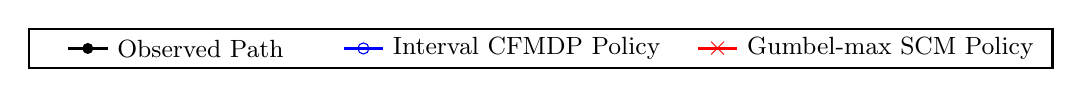
\begin{tikzpicture}[scale=1.0, every node/.style={scale=1.0}]
            \draw[thick, black] (-3, -0.25) rectangle (10, 0.25);
            %
            \draw[black, line width=1pt] (-2.5, 0.0) -- (-2,0.0);
            \fill[black] (-2.25,0.0) circle (2pt); %
            \node[right] at (-2,0.0) {\small Observed Path};
            
            %
            \draw[blue, line width=1pt] (1.0,0.0) -- (1.5,0.0);
            \node[draw=blue, circle, minimum size=4pt, inner sep=0pt] at (1.25,0.0) {}; %
            \node[right] at (1.5,0.0) {\small Interval CFMDP Policy};
            
            %
            \draw[red, line width=1pt] (5.5,0) -- (6,0);
            \node[red] at (5.75,0) {$\boldsymbol{\times}$}; %
            \node[right] at (6,0) {\small Gumbel-max SCM Policy};
        \end{tikzpicture}
    }\\
    %
    \subfigure[\footnotesize Lowest cumulative reward: Interval CFMDP ($312$), Gumbel-max SCM ($312$)]{%
        \resizebox{0.76\columnwidth}{!}{
             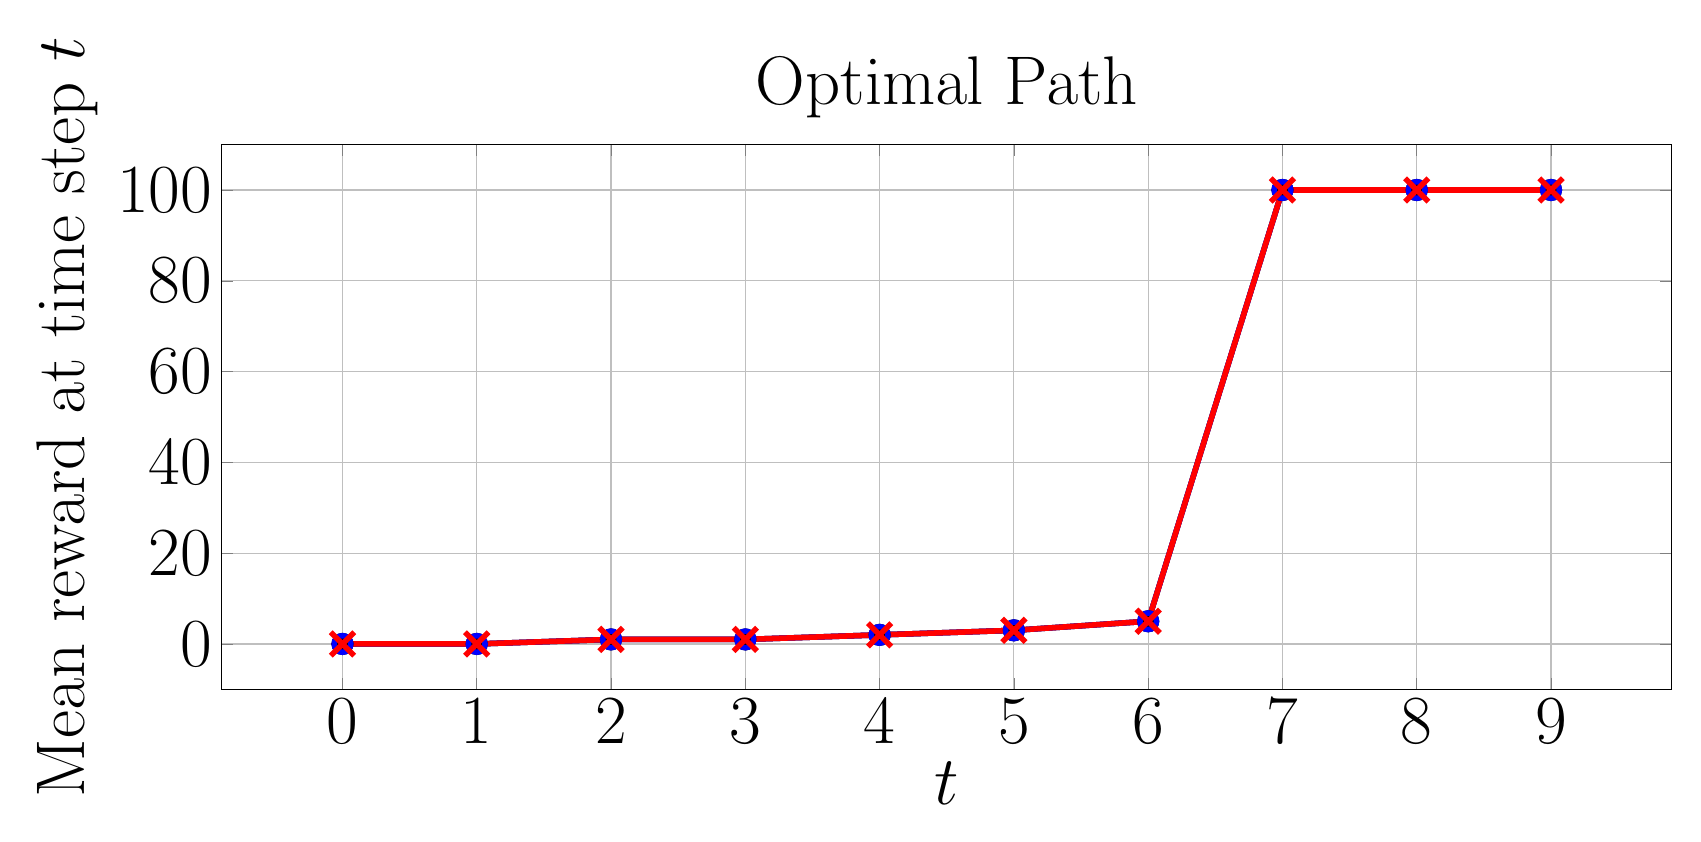
\begin{tikzpicture}
                \begin{axis}[
                    xlabel={$t$},
                    ylabel={Mean reward at time step $t$},
                    title={Optimal Path},
                    grid=both,
                    width=20cm, height=8.5cm,
                    every axis/.style={font=\Huge},
                    %
                ]
                \addplot[
                    color=black, %
                    mark=*, %
                    line width=2pt,
                    mark size=3pt,
                    error bars/.cd,
                    y dir=both, %
                    y explicit, %
                    error bar style={line width=1pt,solid},
                    error mark options={line width=1pt,mark size=4pt,rotate=90}
                ]
                coordinates {
                    (0, 0.0)  +- (0, 0.0)
                    (1, 0.0)  +- (0, 0.0) 
                    (2, 1.0)  +- (0, 0.0) 
                    (3, 1.0)  +- (0, 0.0)
                    (4, 2.0)  +- (0, 0.0)
                    (5, 3.0) +- (0, 0.0)
                    (6, 5.0) +- (0, 0.0)
                    (7, 100.0) +- (0, 0.0)
                    (8, 100.0) +- (0, 0.0)
                    (9, 100.0) +- (0, 0.0)
                };
                %
                \addplot[
                    color=blue, %
                    mark=o, %
                    line width=2pt,
                    mark size=3pt,
                    error bars/.cd,
                    y dir=both, %
                    y explicit, %
                    error bar style={line width=1pt,solid},
                    error mark options={line width=1pt,mark size=4pt,rotate=90}
                ]
                 coordinates {
                    (0, 0.0)  +- (0, 0.0)
                    (1, 0.0)  +- (0, 0.0) 
                    (2, 1.0)  +- (0, 0.0) 
                    (3, 1.0)  +- (0, 0.0)
                    (4, 2.0)  +- (0, 0.0)
                    (5, 3.0) +- (0, 0.0)
                    (6, 5.0) +- (0, 0.0)
                    (7, 100.0) +- (0, 0.0)
                    (8, 100.0) +- (0, 0.0)
                    (9, 100.0) +- (0, 0.0)
                };
                %
                \addplot[
                    color=red, %
                    mark=x, %
                    line width=2pt,
                    mark size=6pt,
                    error bars/.cd,
                    y dir=both, %
                    y explicit, %
                    error bar style={line width=1pt,solid},
                    error mark options={line width=1pt,mark size=4pt,rotate=90}
                ]
                coordinates {
                    (0, 0.0)  +- (0, 0.0)
                    (1, 0.0)  +- (0, 0.0) 
                    (2, 1.0)  +- (0, 0.0) 
                    (3, 1.0)  +- (0, 0.0)
                    (4, 2.0)  +- (0, 0.0)
                    (5, 3.0) +- (0, 0.0)
                    (6, 5.0) +- (0, 0.0)
                    (7, 100.0) +- (0, 0.0)
                    (8, 100.0) +- (0, 0.0)
                    (9, 100.0) +- (0, 0.0)
                };
                \end{axis}
            \end{tikzpicture}
         }
    }
    \hspace{1cm}
    \subfigure[\footnotesize Lowest cumulative reward: Interval CFMDP ($19$), Gumbel-max SCM ($-88$)]{%
         \resizebox{0.76\columnwidth}{!}{
            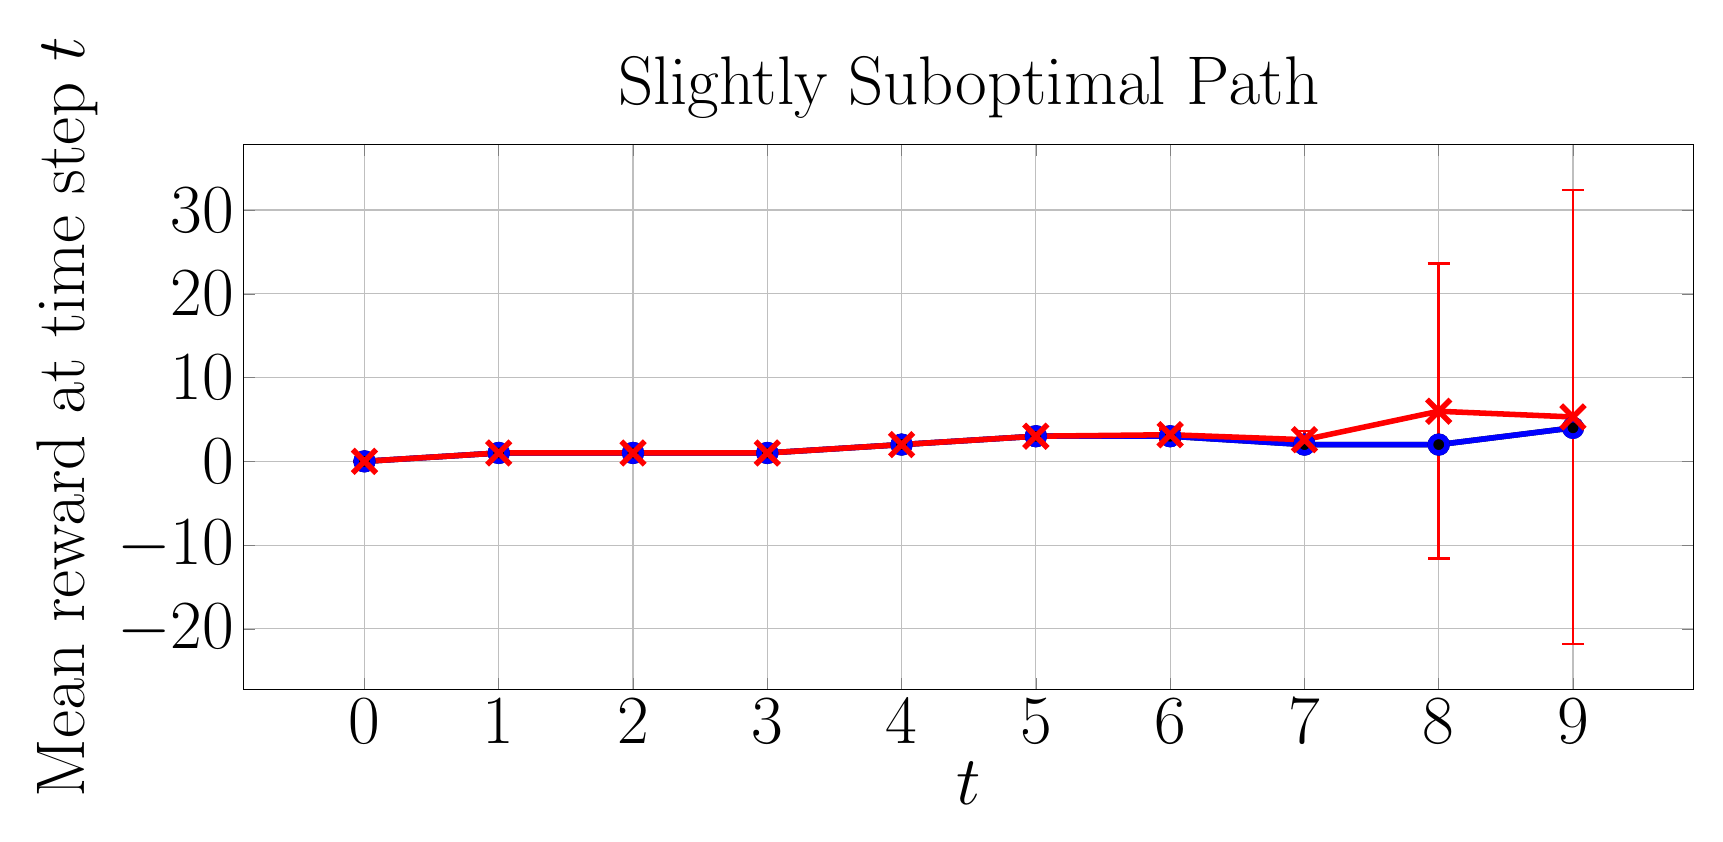
\begin{tikzpicture}
                \begin{axis}[
                    xlabel={$t$},
                    ylabel={Mean reward at time step $t$},
                    title={Slightly Suboptimal Path},
                    grid=both,
                    width=20cm, height=8.5cm,
                    every axis/.style={font=\Huge},
                    %
                ]
                \addplot[
                    color=black, %
                    mark=*, %
                    line width=2pt,
                    mark size=3pt,
                    error bars/.cd,
                    y dir=both, %
                    y explicit, %
                    error bar style={line width=1pt,solid},
                    error mark options={line width=1pt,mark size=4pt,rotate=90}
                ]
              coordinates {
                    (0, 0.0)  +- (0, 0.0)
                    (1, 1.0)  +- (0, 0.0) 
                    (2, 1.0)  +- (0, 0.0) 
                    (3, 1.0)  +- (0, 0.0)
                    (4, 2.0)  +- (0, 0.0)
                    (5, 3.0) +- (0, 0.0)
                    (6, 3.0) +- (0, 0.0)
                    (7, 2.0) +- (0, 0.0)
                    (8, 2.0) +- (0, 0.0)
                    (9, 4.0) +- (0, 0.0)
                };
                %
                \addplot[
                    color=blue, %
                    mark=o, %
                    line width=2pt,
                    mark size=3pt,
                    error bars/.cd,
                    y dir=both, %
                    y explicit, %
                    error bar style={line width=1pt,solid},
                    error mark options={line width=1pt,mark size=4pt,rotate=90}
                ]
              coordinates {
                    (0, 0.0)  +- (0, 0.0)
                    (1, 1.0)  +- (0, 0.0) 
                    (2, 1.0)  +- (0, 0.0) 
                    (3, 1.0)  +- (0, 0.0)
                    (4, 2.0)  +- (0, 0.0)
                    (5, 3.0) +- (0, 0.0)
                    (6, 3.0) +- (0, 0.0)
                    (7, 2.0) +- (0, 0.0)
                    (8, 2.0) +- (0, 0.0)
                    (9, 4.0) +- (0, 0.0)
                };
                %
                \addplot[
                    color=red, %
                    mark=x, %
                    line width=2pt,
                    mark size=6pt,
                    error bars/.cd,
                    y dir=both, %
                    y explicit, %
                    error bar style={line width=1pt,solid},
                    error mark options={line width=1pt,mark size=4pt,rotate=90}
                ]
                coordinates {
                    (0, 0.0)  +- (0, 0.0)
                    (1, 1.0)  +- (0, 0.0) 
                    (2, 1.0)  +- (0, 0.0) 
                    (3, 1.0)  +- (0, 0.0)
                    (4, 2.0)  += (0, 0.0)
                    (5, 3.0)  += (0, 0.0)
                    (6, 3.17847) += (0, 0.62606746) -= (0, 0.62606746)
                    (7, 2.5832885) += (0, 1.04598233) -= (0, 1.04598233)
                    (8, 5.978909) += (0, 17.60137623) -= (0, 17.60137623)
                    (9, 5.297059) += (0, 27.09227512) -= (0, 27.09227512)
                };
                \end{axis}
            \end{tikzpicture}
         }
    }\\[-1.5pt]
    \subfigure[\footnotesize Lowest cumulative reward: Interval CFMDP ($14$), Gumbel-max SCM ($-598$)]{%
         \resizebox{0.76\columnwidth}{!}{
             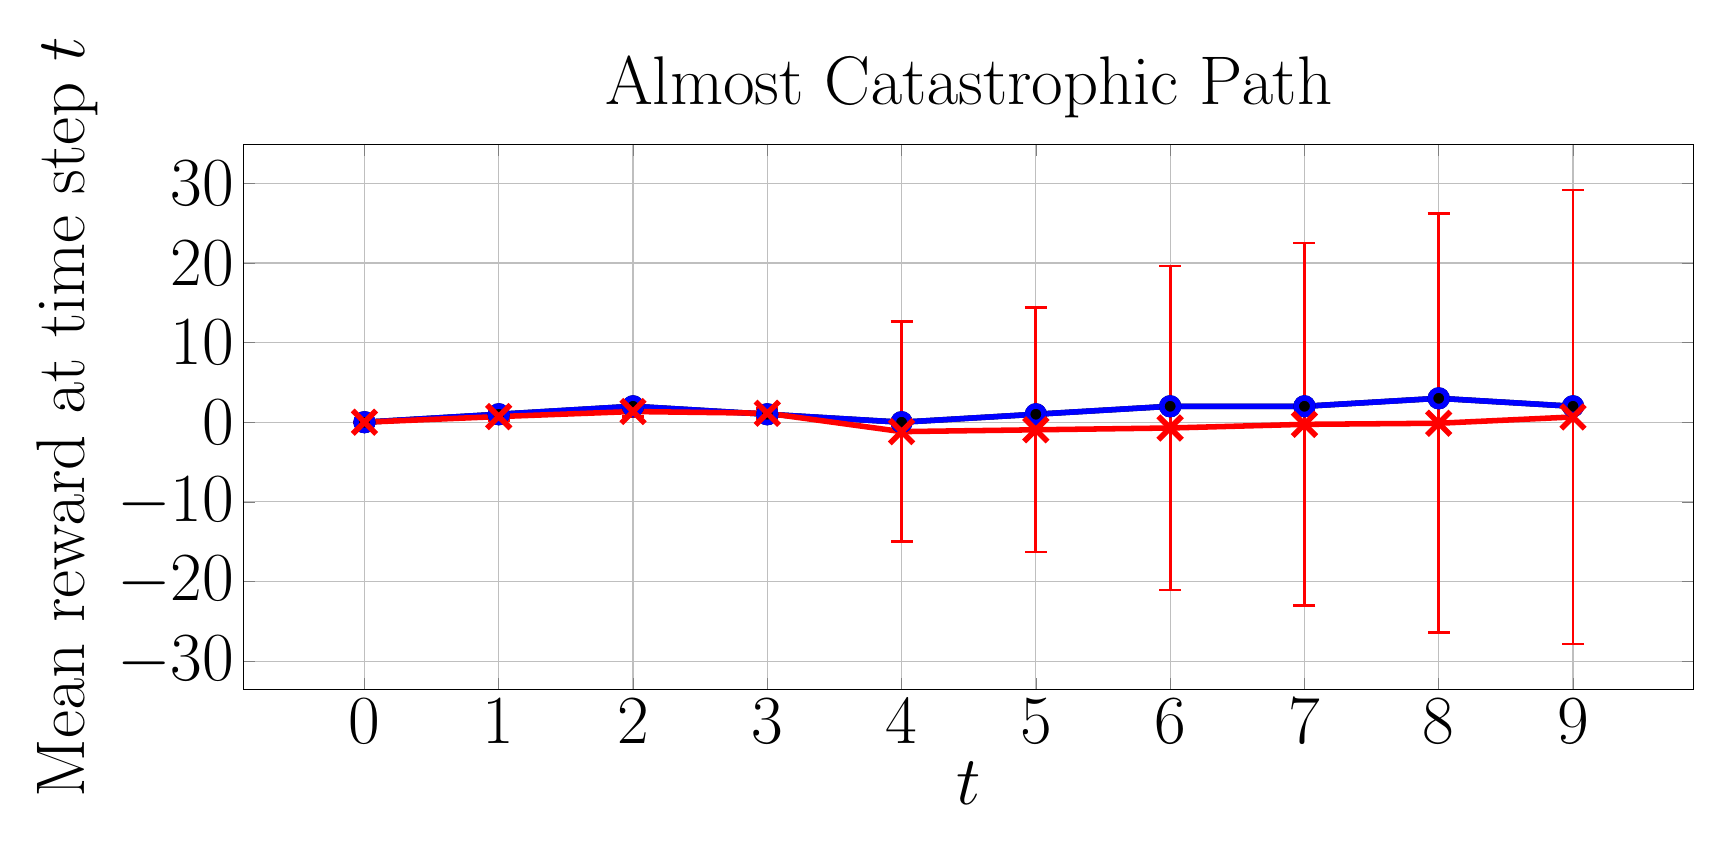
\begin{tikzpicture}
                \begin{axis}[
                    xlabel={$t$},
                    ylabel={Mean reward at time step $t$},
                    title={Almost Catastrophic Path},
                    grid=both,
                    width=20cm, height=8.5cm,
                    every axis/.style={font=\Huge},
                    %
                ]
                \addplot[
                    color=black, %
                    mark=*, %
                    line width=2pt,
                    mark size=3pt,
                    error bars/.cd,
                    y dir=both, %
                    y explicit, %
                    error bar style={line width=1pt,solid},
                    error mark options={line width=1pt,mark size=4pt,rotate=90}
                ]
                coordinates {
                    (0, 0.0)  +- (0, 0.0)
                    (1, 1.0)  +- (0, 0.0) 
                    (2, 2.0)  +- (0, 0.0) 
                    (3, 1.0)  +- (0, 0.0)
                    (4, 0.0)  +- (0, 0.0)
                    (5, 1.0) +- (0, 0.0)
                    (6, 2.0) +- (0, 0.0)
                    (7, 2.0) +- (0, 0.0)
                    (8, 3.0) +- (0, 0.0)
                    (9, 2.0) +- (0, 0.0)
                };
                %
                \addplot[
                    color=blue, %
                    mark=o, %
                    line width=2pt,
                    mark size=3pt,
                    error bars/.cd,
                    y dir=both, %
                    y explicit, %
                    error bar style={line width=1pt,solid},
                    error mark options={line width=1pt,mark size=4pt,rotate=90}
                ]
                coordinates {
                    (0, 0.0)  +- (0, 0.0)
                    (1, 1.0)  +- (0, 0.0) 
                    (2, 2.0)  +- (0, 0.0) 
                    (3, 1.0)  +- (0, 0.0)
                    (4, 0.0)  +- (0, 0.0)
                    (5, 1.0) +- (0, 0.0)
                    (6, 2.0) +- (0, 0.0)
                    (7, 2.0) +- (0, 0.0)
                    (8, 3.0) +- (0, 0.0)
                    (9, 2.0) +- (0, 0.0)
                };
                %
                \addplot[
                    color=red, %
                    mark=x, %
                    line width=2pt,
                    mark size=6pt,
                    error bars/.cd,
                    y dir=both, %
                    y explicit, %
                    error bar style={line width=1pt,solid},
                    error mark options={line width=1pt,mark size=4pt,rotate=90}
                ]
                coordinates {
                    (0, 0.0)  +- (0, 0.0)
                    (1, 0.7065655)  +- (0, 0.4553358) 
                    (2, 1.341673)  +- (0, 0.67091621) 
                    (3, 1.122926)  +- (0, 0.61281824)
                    (4, -1.1821935)  +- (0, 13.82444042)
                    (5, -0.952399)  +- (0, 15.35195457)
                    (6, -0.72672) +- (0, 20.33508414)
                    (7, -0.268983) +- (0, 22.77861454)
                    (8, -0.1310835) +- (0, 26.31013314)
                    (9, 0.65806) +- (0, 28.50670214)
                };
                %
            %
            %
            %
            %
            %
            %
            %
            %
            %
            %
            %
            %
            %
            %
            %
            %
            %
            %
                \end{axis}
            \end{tikzpicture}
         }
    }
    \hspace{1cm}
    \subfigure[\footnotesize Lowest cumulative reward: Interval CFMDP ($-698$), Gumbel-max SCM ($-698$)]{%
         \resizebox{0.76\columnwidth}{!}{
            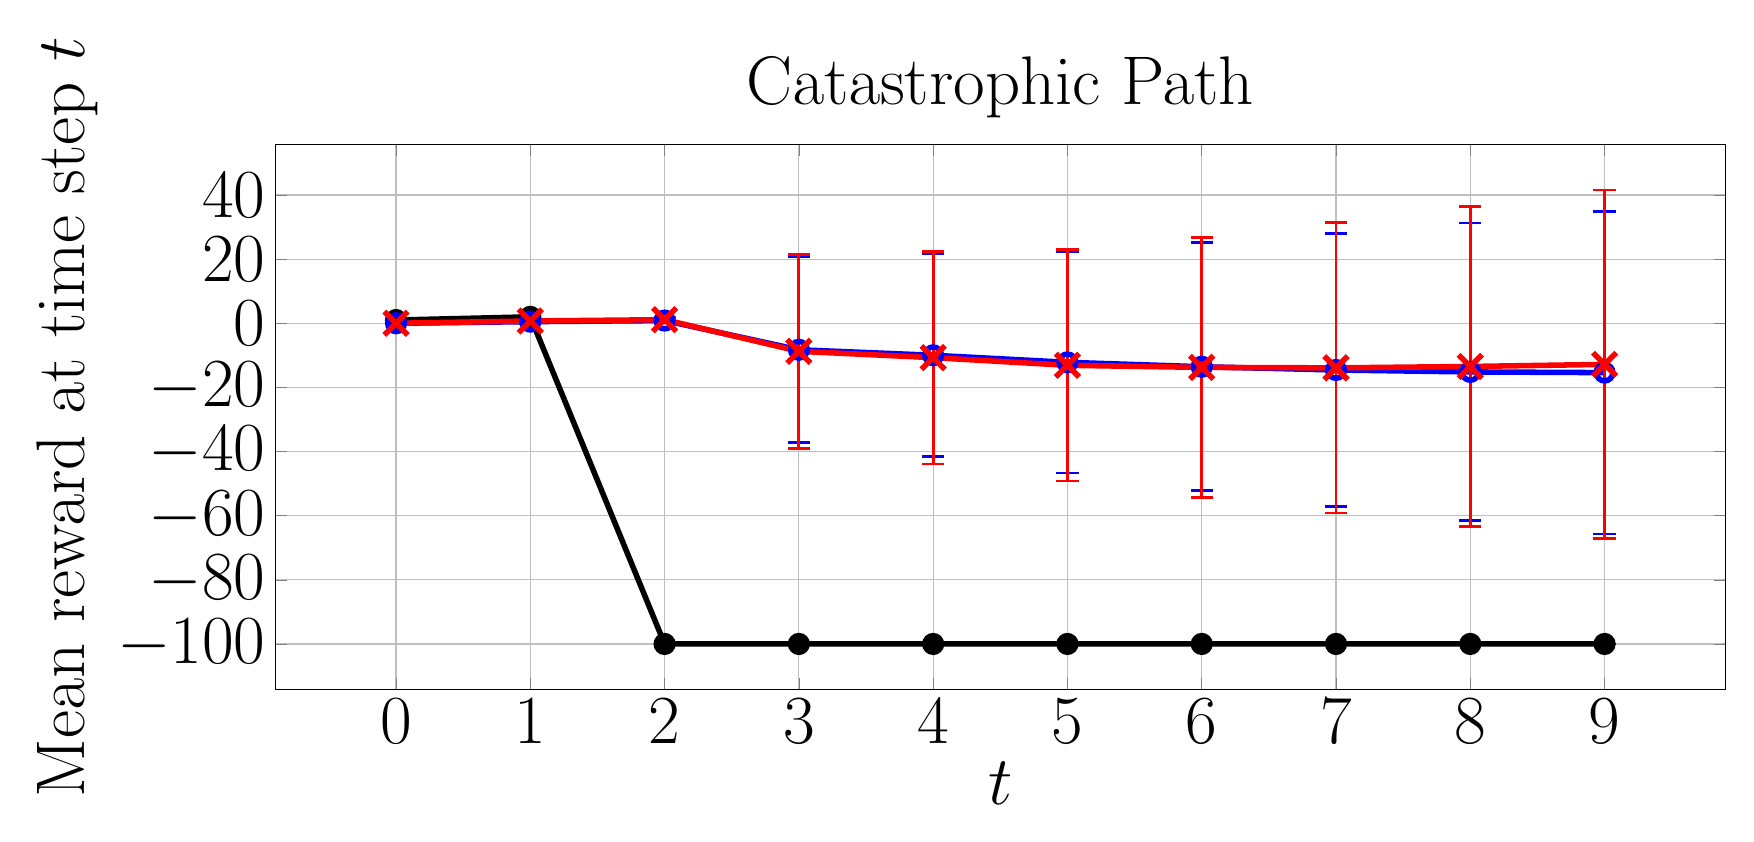
\begin{tikzpicture}
                \begin{axis}[
                    xlabel={$t$},
                    ylabel={Mean reward at time step $t$},
                    title={Catastrophic Path},
                    grid=both,
                    width=20cm, height=8.5cm,
                    every axis/.style={font=\Huge},
                    %
                ]
                \addplot[
                    color=black, %
                    mark=*, %
                    line width=2pt,
                    mark size=3pt,
                    error bars/.cd,
                    y dir=both, %
                    y explicit, %
                    error bar style={line width=1pt,solid},
                    error mark options={line width=1pt,mark size=4pt,rotate=90}
                ]
                coordinates {
                    (0, 1.0)  +- (0, 0.0)
                    (1, 2.0)  +- (0, 0.0) 
                    (2, -100.0)  +- (0, 0.0) 
                    (3, -100.0)  +- (0, 0.0)
                    (4, -100.0)  +- (0, 0.0)
                    (5, -100.0) +- (0, 0.0)
                    (6, -100.0) +- (0, 0.0)
                    (7, -100.0) +- (0, 0.0)
                    (8, -100.0) +- (0, 0.0)
                    (9, -100.0) +- (0, 0.0)
                };
                %
                \addplot[
                    color=blue, %
                    mark=o, %
                    line width=2pt,
                    mark size=3pt,
                    error bars/.cd,
                    y dir=both, %
                    y explicit, %
                    error bar style={line width=1pt,solid},
                    error mark options={line width=1pt,mark size=4pt,rotate=90}
                ]
                coordinates {
                    (0, 0.0)  +- (0, 0.0)
                    (1, 0.504814)  +- (0, 0.49997682) 
                    (2, 0.8439835)  +- (0, 0.76831917) 
                    (3, -8.2709165)  +- (0, 28.93656754)
                    (4, -9.981082)  +- (0, 31.66825363)
                    (5, -12.1776325) +- (0, 34.53463233)
                    (6, -13.556076) +- (0, 38.62845372)
                    (7, -14.574418) +- (0, 42.49603359)
                    (8, -15.1757075) +- (0, 46.41913968)
                    (9, -15.3900395) +- (0, 50.33563368)
                };
                %
                \addplot[
                    color=red, %
                    mark=x, %
                    line width=2pt,
                    mark size=6pt,
                    error bars/.cd,
                    y dir=both, %
                    y explicit, %
                    error bar style={line width=1pt,solid},
                    error mark options={line width=1pt,mark size=4pt,rotate=90}
                ]
                coordinates {
                    (0, 0.0)  +- (0, 0.0)
                    (1, 0.701873)  +- (0, 0.45743556) 
                    (2, 1.1227805)  +- (0, 0.73433129) 
                    (3, -8.7503255)  +- (0, 30.30257976)
                    (4, -10.722092)  +- (0, 33.17618589)
                    (5, -13.10721)  +- (0, 36.0648089)
                    (6, -13.7631645) +- (0, 40.56553451)
                    (7, -13.909043) +- (0, 45.23829402)
                    (8, -13.472517) +- (0, 49.96270296)
                    (9, -12.8278835) +- (0, 54.38618735)
                };
                %
            %
            %
            %
            %
            %
            %
            %
            %
            %
            %
            %
            %
            %
            %
            %
            %
            %
            %
                \end{axis}
            \end{tikzpicture}
         }
    }
    \caption{Average instant reward of CF paths induced by policies on GridWorld $p=0.4$.}
    \label{fig: reward p=0.4}
\end{figure*}

\subsection{Experimental Setup}
To compare policy performance, we measure the average rewards of counterfactual paths induced by our policy and the Gumbel-max policy by uniformly sampling $200$ counterfactual MDPs from the ICFMDP and generating $10,000$ counterfactual paths over each sampled CFMDP. \jl{Since the interval CFMDP depends on the observed path, we select $4$  paths of varying optimality to evaluate how the observed path impacts the performance of both policies: an optimal path, a slightly suboptimal path that could reach the optimal reward with a few changes, a catastrophic path that enters a catastrophic, terminal state with low reward, and an almost catastrophic path that was close to entering a catastrophic state.} When measuring the average probability bound widths and execution time needed to generate the ICFMDPs, we averaged over $20$ randomly generated observed paths
\footnote{Further training details are provided in Appendix \ref{app: training details}, and the code is provided at \href{https://github.com/ddv-lab/robust-cf-inference-in-MDPs}{https://github.com/ddv-lab/robust-cf-inference-in-MDPs}
%
%
.}.

\subsection{GridWorld}
\jl{The GridWorld MDP is a $4 \times 4$ grid where an agent must navigate from the top-left corner to the goal state in the bottom-right corner, avoiding a dangerous terminal state in the centre. At each time step, the agent can move up, down, left, or right, but there is a small probability (controlled by hyper-parameter $p$) of moving in an unintended direction. As the agent nears the goal, the reward for each state increases, culminating in a reward of $+100$ for reaching the goal. Entering the dangerous state results in a penalty of $-100$. We use two versions of GridWorld: a less stochastic version with $p=0.9$ (i.e., $90$\% chance of moving in the chosen direction) and a more stochastic version with $p=0.4$.}

\paragraph{GridWorld ($p=0.9$)}
When $p=0.9$, the counterfactual probability bounds are typically narrow (see Table \ref{tab:nonzero_probs} for average measurements). Consequently, as shown in Figure \ref{fig: reward p=0.9}, both policies are nearly identical and perform similarly well across the optimal, slightly suboptimal, and catastrophic paths.
%
However, for the almost catastrophic path, the interval CFMDP path is more conservative and follows the observed path more closely (as this is where the probability bounds are narrowest), which typically requires one additional step to reach the goal state than the Gumbel-max SCM policy.
%

\paragraph{GridWorld ($p=0.4$)}
\jl{When $p=0.4$, the GridWorld environment becomes more uncertain, increasing the risk of entering the dangerous state even if correct actions are chosen. Thus, as shown in Figure \ref{fig: reward p=0.4}, the interval CFMDP policy adopts a more conservative approach, avoiding deviation from the observed policy if it cannot guarantee higher counterfactual rewards (see the slightly suboptimal and almost catastrophic paths), whereas the Gumbel-max SCM is inconsistent: it can yield higher rewards, but also much lower rewards, reflected in the wide error bars.} For the catastrophic path, both policies must deviate from the observed path to achieve a higher reward and, in this case, perform similarly.
%
%
%
%
\subsection{Sepsis}
The Sepsis MDP \citep{oberst2019counterfactual} simulates trajectories of Sepsis patients. Each state consists of four vital signs (heart rate, blood pressure, oxygen concentration, and glucose levels), categorised as low, normal, or high.
and three treatments that can be toggled on/off at each time step (8 actions in total). Unlike \citet{oberst2019counterfactual}, we scale rewards based on the number of out-of-range vital signs, between $-1000$ (patient dies) and $1000$ (patient discharged). \jl{Like the GridWorld $p=0.4$ experiment, the Sepsis MDP is highly uncertain, as many states are equally likely to lead to optimal and poor outcomes. Thus, as shown in Figure \ref{fig: reward sepsis}, both policies follow the observed optimal and almost catastrophic paths to guarantee rewards are no worse than the observation.} However, improving the catastrophic path requires deviating from the observation. Here, the Gumbel-max SCM policy, on average, performs better than the interval CFMDP policy. But, since both policies have lower bounds clipped at $-1000$, neither policy reliably improves over the observation. In contrast, for the slightly suboptimal path, the interval CFMDP policy performs significantly better, shown by its higher lower bounds. 
Moreover, in these two cases, the worst-case counterfactual path generated by the interval CFMDP policy is better than that of the Gumbel-max SCM policy,
indicating its greater robustness.
%
\begin{figure*}
    \centering
     \resizebox{0.6\textwidth}{!}{
        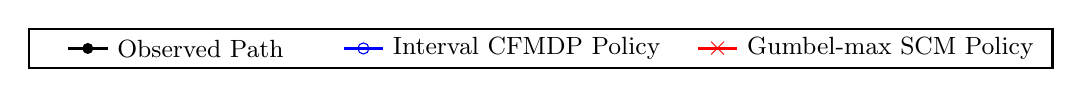
\begin{tikzpicture}[scale=1.0, every node/.style={scale=1.0}]
            \draw[thick, black] (-3, -0.25) rectangle (10, 0.25);
            %
            \draw[black, line width=1pt] (-2.5, 0.0) -- (-2,0.0);
            \fill[black] (-2.25,0.0) circle (2pt); %
            \node[right] at (-2,0.0) {\small Observed Path};
            
            %
            \draw[blue, line width=1pt] (1.0,0.0) -- (1.5,0.0);
            \node[draw=blue, circle, minimum size=4pt, inner sep=0pt] at (1.25,0.0) {}; %
            \node[right] at (1.5,0.0) {\small Interval CFMDP Policy};
            
            %
            \draw[red, line width=1pt] (5.5,0) -- (6,0);
            \node[red] at (5.75,0) {$\boldsymbol{\times}$}; %
            \node[right] at (6,0) {\small Gumbel-max SCM Policy};
        \end{tikzpicture}
    }\\
    \subfigure[\footnotesize Lowest cumulative reward: Interval CFMDP ($8000$), Gumbel-max SCM ($8000$)]{%
         \resizebox{0.76\columnwidth}{!}{
             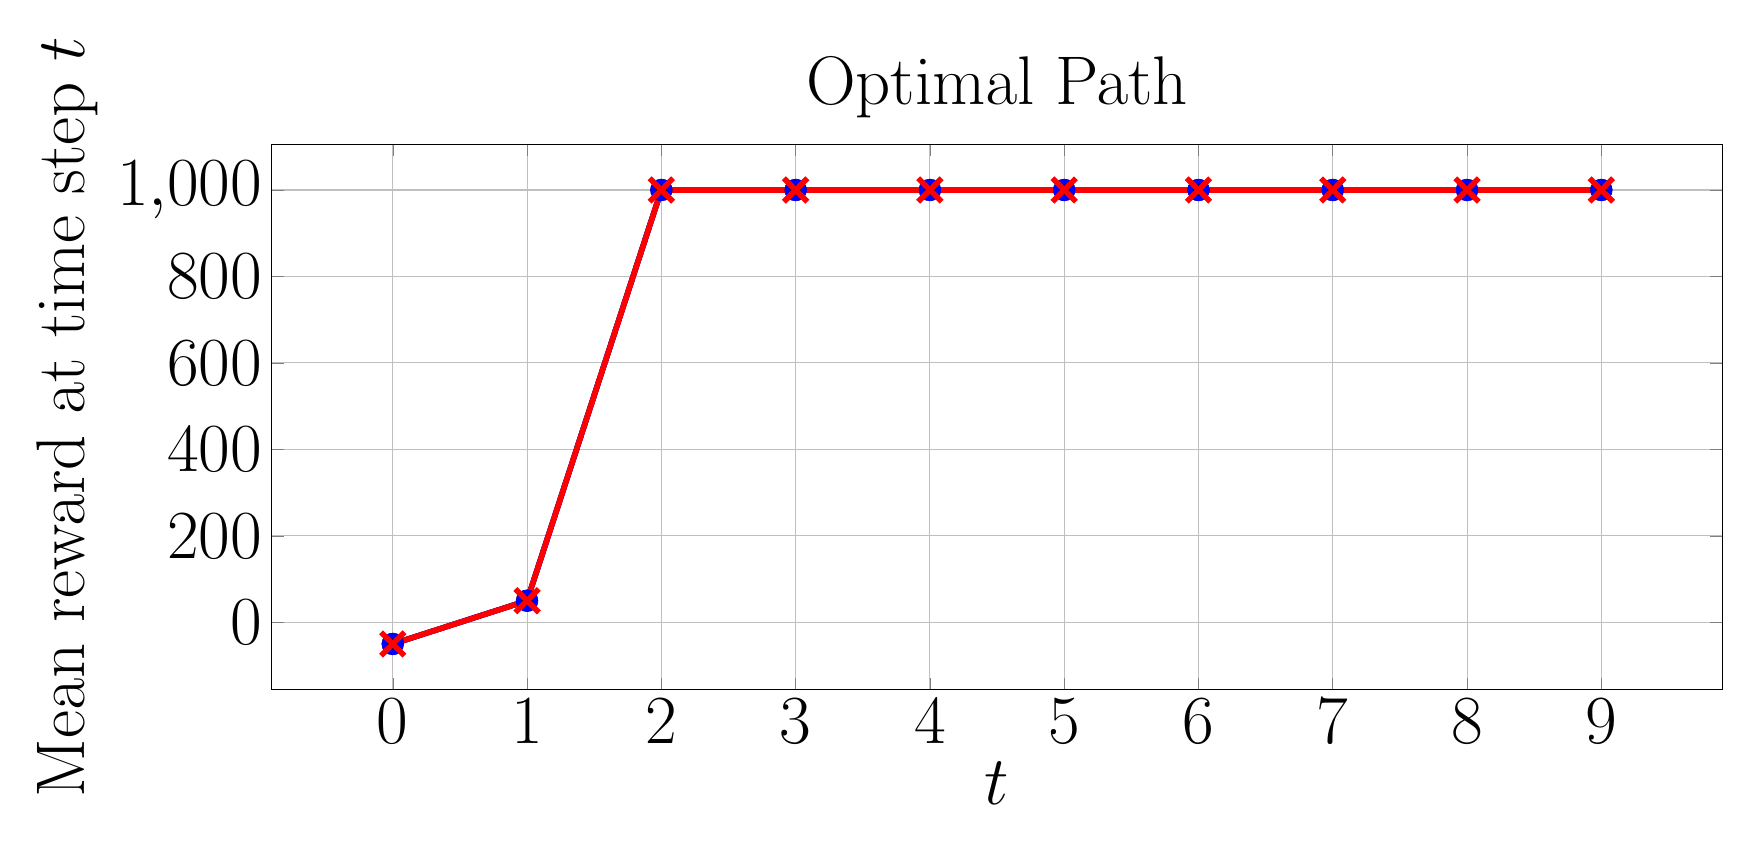
\begin{tikzpicture}
                \begin{axis}[
                    xlabel={$t$},
                    ylabel={Mean reward at time step $t$},
                    title={Optimal Path},
                    grid=both,
                    width=20cm, height=8.5cm,
                    every axis/.style={font=\Huge},
                    %
                ]
                \addplot[
                    color=black, %
                    mark=*, %
                    line width=2pt,
                    mark size=3pt,
                ]
                coordinates {
                    (0, -50.0)
                    (1, 50.0)
                    (2, 1000.0)
                    (3, 1000.0)
                    (4, 1000.0)
                    (5, 1000.0)
                    (6, 1000.0)
                    (7, 1000.0)
                    (8, 1000.0)
                    (9, 1000.0)
                };
                %
                \addplot[
                    color=blue, %
                    mark=o, %
                    line width=2pt,
                    mark size=3pt,
                    error bars/.cd,
                    y dir=both, %
                    y explicit, %
                    error bar style={line width=1pt,solid},
                    error mark options={line width=1pt,mark size=4pt,rotate=90}
                ]
                coordinates {
                    (0, -50.0)  +- (0, 0.0)
                    (1, 50.0)  +- (0, 0.0) 
                    (2, 1000.0)  +- (0, 0.0) 
                    (3, 1000.0)  +- (0, 0.0)
                    (4, 1000.0)  +- (0, 0.0)
                    (5, 1000.0) +- (0, 0.0)
                    (6, 1000.0) +- (0, 0.0)
                    (7, 1000.0) +- (0, 0.0)
                    (8, 1000.0) +- (0, 0.0)
                    (9, 1000.0) +- (0, 0.0)
                };
                %
                \addplot[
                    color=red, %
                    mark=x, %
                    line width=2pt,
                    mark size=6pt,
                    error bars/.cd,
                    y dir=both, %
                    y explicit, %
                    error bar style={line width=1pt,solid},
                    error mark options={line width=1pt,mark size=4pt,rotate=90}
                ]
                coordinates {
                    (0, -50.0)  +- (0, 0.0)
                    (1, 50.0)  +- (0, 0.0) 
                    (2, 1000.0)  +- (0, 0.0) 
                    (3, 1000.0)  +- (0, 0.0)
                    (4, 1000.0)  +- (0, 0.0)
                    (5, 1000.0) +- (0, 0.0)
                    (6, 1000.0) +- (0, 0.0)
                    (7, 1000.0) +- (0, 0.0)
                    (8, 1000.0) +- (0, 0.0)
                    (9, 1000.0) +- (0, 0.0)
                };
                %
                \end{axis}
            \end{tikzpicture}
         }
    }
    \hspace{1cm}
    \subfigure[\footnotesize Lowest cumulative reward: Interval CFMDP ($-5980$), Gumbel-max SCM ($-8000$)]{%
         \resizebox{0.76\columnwidth}{!}{
            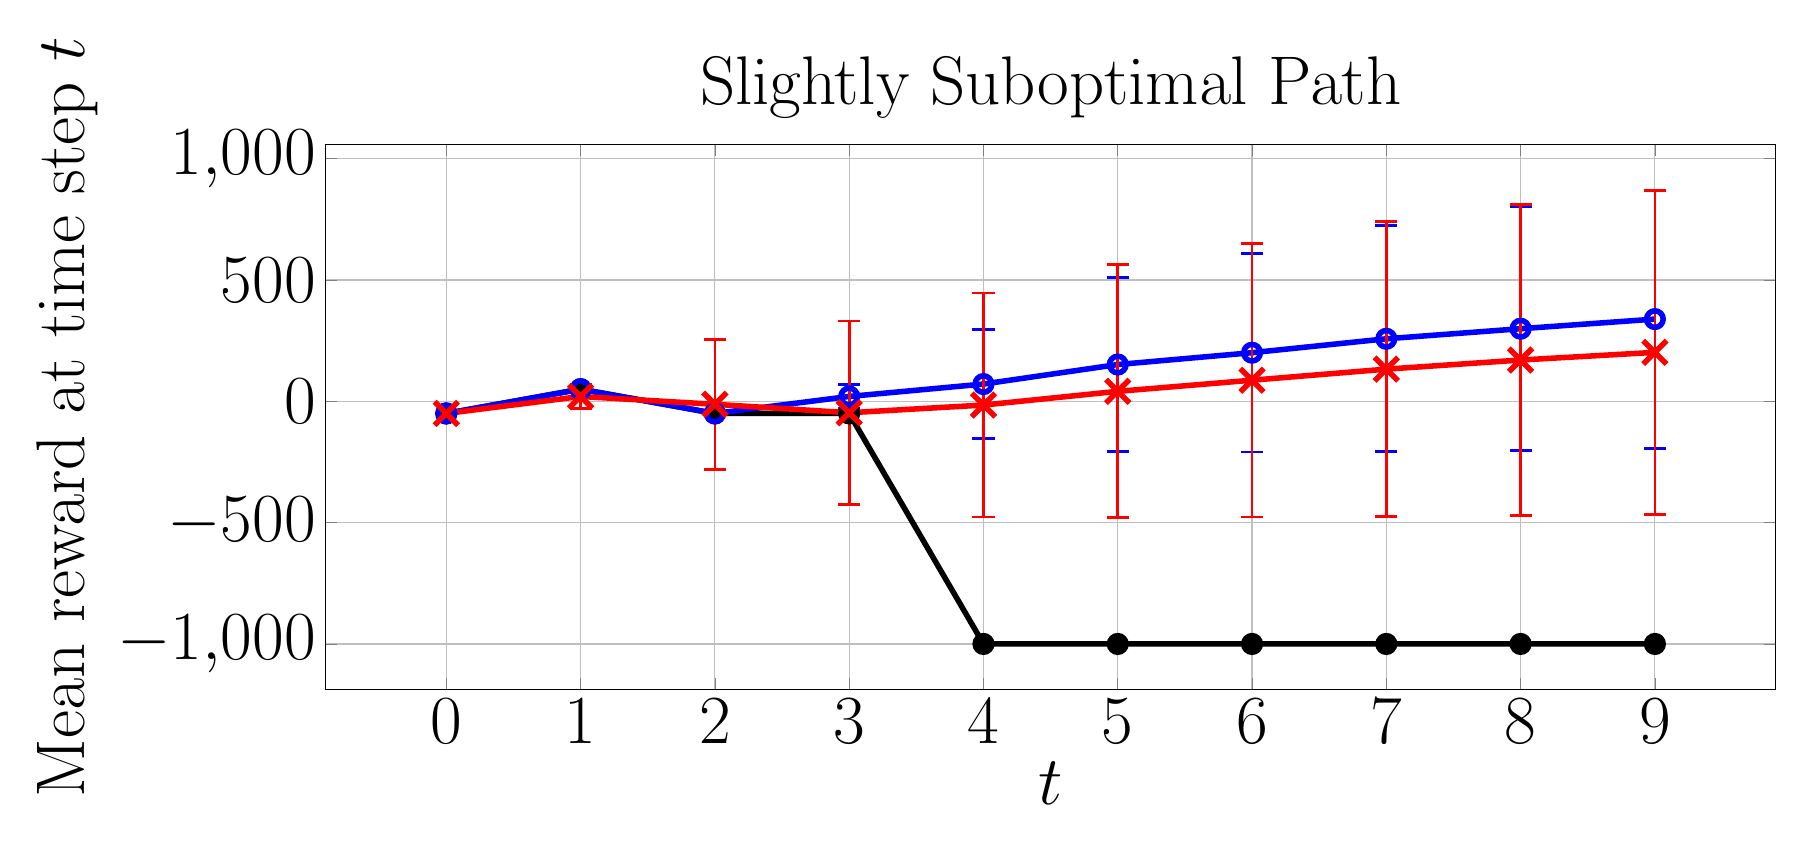
\begin{tikzpicture}
                \begin{axis}[
                    xlabel={$t$},
                    ylabel={Mean reward at time step $t$},
                    title={Slightly Suboptimal Path},
                    grid=both,
                    width=20cm, height=8.5cm,
                    every axis/.style={font=\Huge},
                    %
                ]
               \addplot[
                    color=black, %
                    mark=*, %
                    line width=2pt,
                    mark size=3pt,
                ]
                coordinates {
                    (0, -50.0)
                    (1, 50.0)
                    (2, -50.0)
                    (3, -50.0)
                    (4, -1000.0)
                    (5, -1000.0)
                    (6, -1000.0)
                    (7, -1000.0)
                    (8, -1000.0)
                    (9, -1000.0)
                };
                %
                \addplot[
                    color=blue, %
                    mark=o, %
                    line width=2pt,
                    mark size=3pt,
                    error bars/.cd,
                    y dir=both, %
                    y explicit, %
                    error bar style={line width=1pt,solid},
                    error mark options={line width=1pt,mark size=4pt,rotate=90}
                ]
                coordinates {
                    (0, -50.0)  +- (0, 0.0)
                    (1, 50.0)  +- (0, 0.0) 
                    (2, -50.0)  +- (0, 0.0) 
                    (3, 20.0631)  +- (0, 49.97539413)
                    (4, 71.206585)  +- (0, 226.02033693)
                    (5, 151.60797) +- (0, 359.23292559)
                    (6, 200.40593) +- (0, 408.86185176)
                    (7, 257.77948) +- (0, 466.10372804)
                    (8, 299.237465) +- (0, 501.82579506)
                    (9, 338.9129) +- (0, 532.06124996)
                };
                %
                \addplot[
                    color=red, %
                    mark=x, %
                    line width=2pt,
                    mark size=6pt,
                    error bars/.cd,
                    y dir=both, %
                    y explicit, %
                    error bar style={line width=1pt,solid},
                    error mark options={line width=1pt,mark size=4pt,rotate=90}
                ]
                coordinates {
                    (0, -50.0)  +- (0, 0.0)
                    (1, 20.00736)  +- (0, 49.99786741) 
                    (2, -12.282865)  +- (0, 267.598755) 
                    (3, -47.125995)  +- (0, 378.41755832)
                    (4, -15.381965)  +- (0, 461.77616558)
                    (5, 41.15459) +- (0, 521.53189262)
                    (6, 87.01595) +- (0, 564.22243126 )
                    (7, 132.62376) +- (0, 607.31338037)
                    (8, 170.168145) +- (0, 641.48013693)
                    (9, 201.813135) +- (0, 667.29441777)
                };
                %
                %
                %
                %
                %
                %
                %
                %
                %
                %
                %
                %
                %
                %
                %
                %
                %
                %
                %
                \end{axis}
            \end{tikzpicture}
         }
    }\\[-1.5pt]
    \subfigure[\footnotesize Lowest cumulative reward: Interval CFMDP ($100$), Gumbel-max SCM ($100$)]{%
         \resizebox{0.76\columnwidth}{!}{
             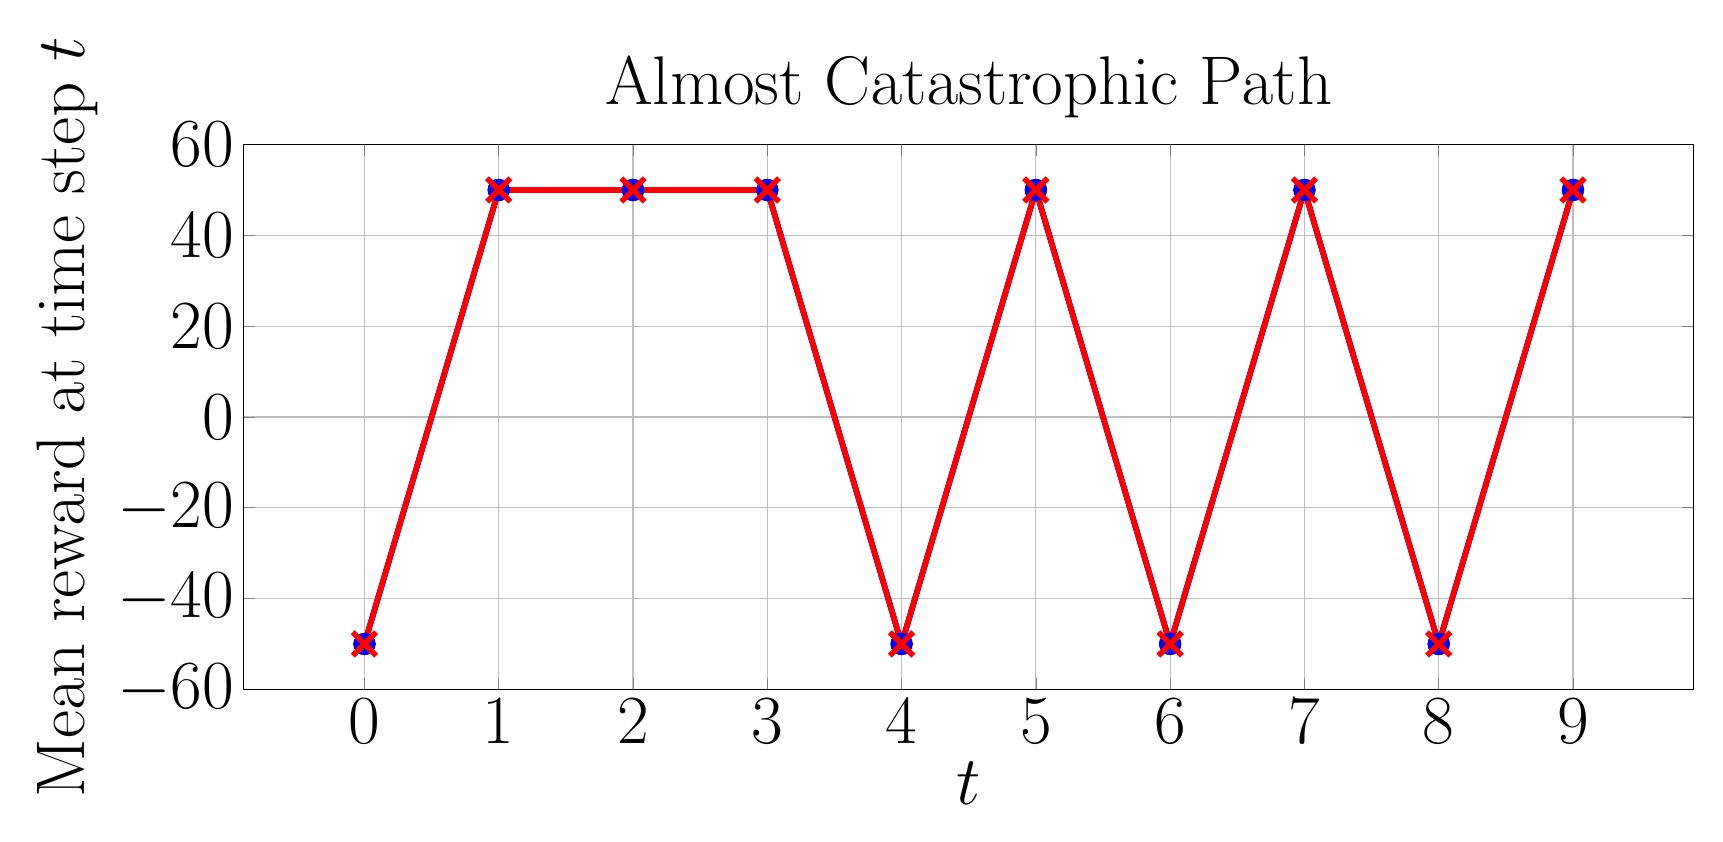
\begin{tikzpicture}
                \begin{axis}[
                    xlabel={$t$},
                    ylabel={Mean reward at time step $t$},
                    title={Almost Catastrophic Path},
                    grid=both,
                    every axis/.style={font=\Huge},
                    width=20cm, height=8.5cm,
                    %
                ]
               \addplot[
                    color=black, %
                    mark=*, %
                    line width=2pt,
                    mark size=3pt,
                ]
                coordinates {
                    (0, -50.0)
                    (1, 50.0)
                    (2, 50.0)
                    (3, 50.0)
                    (4, -50.0)
                    (5, 50.0)
                    (6, -50.0)
                    (7, 50.0)
                    (8, -50.0)
                    (9, 50.0)
                };
                %
                %
                \addplot[
                    color=blue, %
                    mark=o, %
                    line width=2pt,
                    mark size=3pt,
                    error bars/.cd,
                    y dir=both, %
                    y explicit, %
                    error bar style={line width=1pt,solid},
                    error mark options={line width=1pt,mark size=4pt,rotate=90}
                ]
                coordinates {
                    (0, -50.0)  +- (0, 0.0)
                    (1, 50.0)  +- (0, 0.0) 
                    (2, 50.0)  +- (0, 0.0) 
                    (3, 50.0)  +- (0, 0.0)
                    (4, -50.0)  +- (0, 0.0)
                    (5, 50.0) +- (0, 0.0)
                    (6, -50.0) +- (0, 0.0)
                    (7, 50.0) +- (0, 0.0)
                    (8, -50.0) +- (0, 0.0)
                    (9, 50.0) +- (0, 0.0)
                };
                %
                \addplot[
                    color=red, %
                    mark=x, %
                    line width=2pt,
                    mark size=6pt,
                    error bars/.cd,
                    y dir=both, %
                    y explicit, %
                    error bar style={line width=1pt,solid},
                    error mark options={line width=1pt,mark size=4pt,rotate=90}
                ]
                coordinates {
                    (0, -50.0)  +- (0, 0.0)
                    (1, 50.0)  +- (0, 0.0) 
                    (2, 50.0)  +- (0, 0.0) 
                    (3, 50.0)  +- (0, 0.0)
                    (4, -50.0)  +- (0, 0.0)
                    (5, 50.0) +- (0, 0.0)
                    (6, -50.0) +- (0, 0.0)
                    (7, 50.0) +- (0, 0.0)
                    (8, -50.0) +- (0, 0.0)
                    (9, 50.0) +- (0, 0.0)
                };
                %
                %
                %
                %
                %
                %
                %
                %
                %
                %
                %
                %
                %
                %
                %
                %
                %
                %
                %
                \end{axis}
            \end{tikzpicture}
         }
    }
    \hspace{1cm}
    \subfigure[\footnotesize Lowest cumulative reward: Interval CFMDP ($-7150$), Gumbel-max SCM ($-9050$)]{%
         \resizebox{0.76\columnwidth}{!}{
            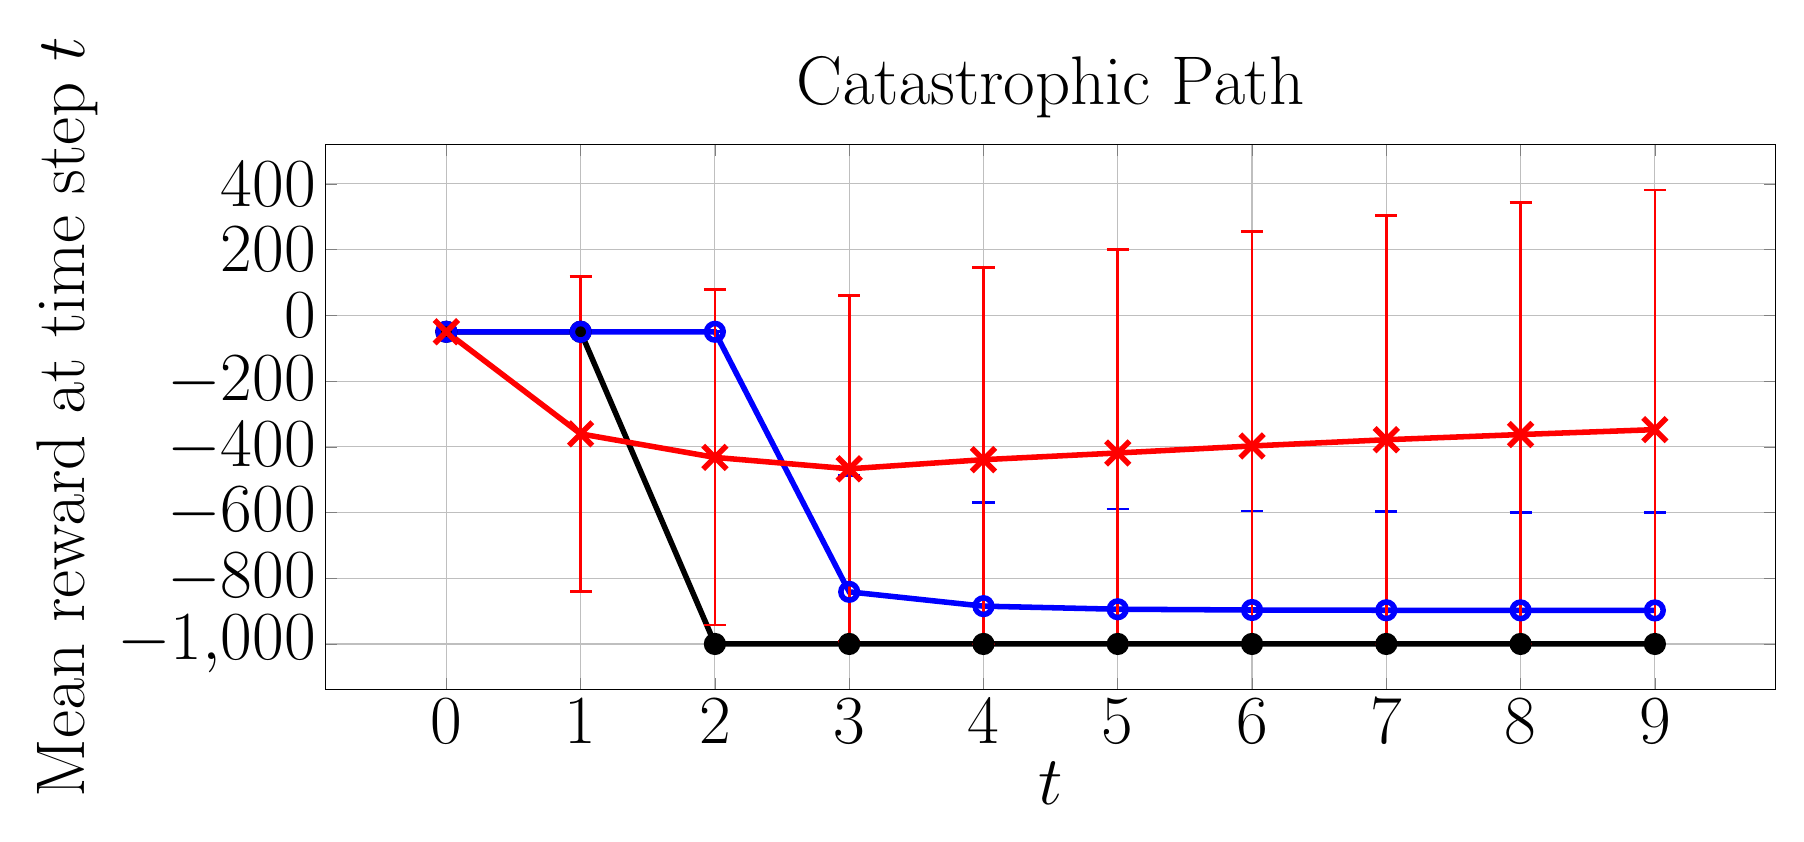
\begin{tikzpicture}
                \begin{axis}[
                    xlabel={$t$},
                    ylabel={Mean reward at time step $t$},
                    title={Catastrophic Path},
                    grid=both,
                    width=20cm, height=8.5cm,
                    every axis/.style={font=\Huge},
                    %
                ]
               \addplot[
                    color=black, %
                    mark=*, %
                    line width=2pt,
                    mark size=3pt,
                ]
                coordinates {
                    (0, -50.0)
                    (1, -50.0)
                    (2, -1000.0)
                    (3, -1000.0)
                    (4, -1000.0)
                    (5, -1000.0)
                    (6, -1000.0)
                    (7, -1000.0)
                    (8, -1000.0)
                    (9, -1000.0)
                };
                %
                %
                \addplot[
                    color=blue, %
                    mark=o, %
                    line width=2pt,
                    mark size=3pt,
                    error bars/.cd,
                    y dir=both, %
                    y explicit, %
                    error bar style={line width=1pt,solid},
                    error mark options={line width=1pt,mark size=4pt,rotate=90}
                ]
                coordinates {
                    (0, -50.0)  +- (0, 0.0)
                    (1, -50.0)  +- (0, 0.0) 
                    (2, -50.0)  +- (0, 0.0) 
                    (3, -841.440725)  += (0, 354.24605512) -= (0, 158.559275)
                    (4, -884.98225)  += (0, 315.37519669) -= (0, 115.01775)
                    (5, -894.330425) += (0, 304.88572805) -= (0, 105.669575)
                    (6, -896.696175) += (0, 301.19954514) -= (0, 103.303825)
                    (7, -897.4635) += (0, 299.61791279) -= (0, 102.5365)
                    (8, -897.77595) += (0, 298.80392585) -= (0, 102.22405)
                    (9, -897.942975) += (0, 298.32920557) -= (0, 102.057025)
                };
                %
                \addplot[
                    color=red, %
                    mark=x, %
                    line width=2pt,
                    mark size=6pt,
                    error bars/.cd,
                    y dir=both, %
                    y explicit, %
                    error bar style={line width=1pt,solid},
                    error mark options={line width=1pt,mark size=4pt,rotate=90}
                ]
            coordinates {
                    (0, -50.0)  +- (0, 0.0)
                    (1, -360.675265)  +- (0, 479.39812699) 
                    (2, -432.27629)  +- (0, 510.38620897) 
                    (3, -467.029545)  += (0, 526.36009628) -= (0, 526.36009628)
                    (4, -439.17429)  += (0, 583.96638919) -= (0, 560.82571)
                    (5, -418.82704) += (0, 618.43027478) -= (0, 581.17296)
                    (6, -397.464895) += (0, 652.67322574) -= (0, 602.535105)
                    (7, -378.49052) += (0, 682.85407033) -= (0, 621.50948)
                    (8, -362.654195) += (0, 707.01412023) -= (0, 637.345805)
                    (9, -347.737935) += (0, 729.29076479) -= (0, 652.262065)
                };
                %
                %
                %
                %
                %
                %
                %
                %
                %
                %
                %
                %
                %
                %
                %
                %
                %
                %
                %
                \end{axis}
            \end{tikzpicture}
         }
    }
    \caption{Average instant reward of CF paths induced by policies on Sepsis.}
    \label{fig: reward sepsis}
\end{figure*}

%
%
%
\subsection{Interval CFMDP Bounds}
%
%
Table \ref{tab:nonzero_probs} presents the mean counterfactual probability bound widths (excluding transitions where the upper bound is $0$) for each MDP, averaged over 20 observed paths. We compare the bounds under counterfactual stability (CS) and monotonicity (M) assumptions, CS alone, and no assumptions. This shows that the assumptions marginally reduce the bound widths, indicating the assumptions tighten the bounds without excluding too many causal models, as intended.
\renewcommand{\arraystretch}{1}

\begin{table}
\centering
\caption{Mean width of counterfactual probability bounds}
\resizebox{0.8\columnwidth}{!}{%
\begin{tabular}{|c|c|c|c|}
\hline
\multirow{2}{*}{\textbf{Environment}} & \multicolumn{3}{c|}{\textbf{Assumptions}} \\ \cline{2-4}
 & \textbf{CS + M} & \textbf{CS} & \textbf{None\tablefootnote{\jl{Equivalent to \citet{li2024probabilities}'s bounds (see Section \ref{sec: equivalence with Li}).}}} \\ \hline
\textbf{GridWorld} ($p=0.9$) & 0.0817 & 0.0977 & 0.100 \\ \hline
\textbf{GridWorld} ($p=0.4$) & 0.552  & 0.638  & 0.646 \\ \hline
\textbf{Sepsis} & 0.138 & 0.140 & 0.140 \\ \hline
\end{tabular}
}
\label{tab:nonzero_probs}
\end{table}


\subsection{Execution Times}
Table \ref{tab: times} compares the average time needed to generate the interval CFMDP vs.\ the Gumbel-max SCM CFMDP for 20 observations.
The GridWorld algorithms were run single-threaded, while the Sepsis experiments were run in parallel.
Generating the interval CFMDP is significantly faster as it uses exact analytical bounds, whereas the Gumbel-max CFMDP requires sampling from the Gumbel distribution to estimate counterfactual transition probabilities. \jl{Since constructing the counterfactual MDP models is the main bottleneck in both approaches, ours is more efficient overall and suitable for larger MDPs.}
\begin{table}
\centering
\caption{Mean execution time to generate CFMDPs}
\resizebox{0.99\columnwidth}{!}{%
\begin{tabular}{|c|c|c|}
\hline
\multirow{2}{*}{\textbf{Environment}} & \multicolumn{2}{c|}{\textbf{Mean Execution Time (s)}} \\ \cline{2-3} 
                                      & \textbf{Interval CFMDP} & \textbf{Gumbel-max CFMDP} \\ \hline
\textbf{GridWorld ($p=0.9$) }                  & 0.261                   & 56.1                      \\ \hline
\textbf{GridWorld ($p=0.4$)  }                 & 0.336                   & 54.5                      \\ \hline
\textbf{Sepsis}                                 & 688                     & 2940                      \\ \hline
\end{tabular}%
}
\label{tab: times}
\end{table}

\section{RELATED WORK}
\label{sec:relatedwork}
In this section, we describe the previous works related to our proposal, which are divided into two parts. In Section~\ref{sec:relatedwork_exoplanet}, we present a review of approaches based on machine learning techniques for the detection of planetary transit signals. Section~\ref{sec:relatedwork_attention} provides an account of the approaches based on attention mechanisms applied in Astronomy.\par

\subsection{Exoplanet detection}
\label{sec:relatedwork_exoplanet}
Machine learning methods have achieved great performance for the automatic selection of exoplanet transit signals. One of the earliest applications of machine learning is a model named Autovetter \citep{MCcauliff}, which is a random forest (RF) model based on characteristics derived from Kepler pipeline statistics to classify exoplanet and false positive signals. Then, other studies emerged that also used supervised learning. \cite{mislis2016sidra} also used a RF, but unlike the work by \citet{MCcauliff}, they used simulated light curves and a box least square \citep[BLS;][]{kovacs2002box}-based periodogram to search for transiting exoplanets. \citet{thompson2015machine} proposed a k-nearest neighbors model for Kepler data to determine if a given signal has similarity to known transits. Unsupervised learning techniques were also applied, such as self-organizing maps (SOM), proposed \citet{armstrong2016transit}; which implements an architecture to segment similar light curves. In the same way, \citet{armstrong2018automatic} developed a combination of supervised and unsupervised learning, including RF and SOM models. In general, these approaches require a previous phase of feature engineering for each light curve. \par

%DL is a modern data-driven technology that automatically extracts characteristics, and that has been successful in classification problems from a variety of application domains. The architecture relies on several layers of NNs of simple interconnected units and uses layers to build increasingly complex and useful features by means of linear and non-linear transformation. This family of models is capable of generating increasingly high-level representations \citep{lecun2015deep}.

The application of DL for exoplanetary signal detection has evolved rapidly in recent years and has become very popular in planetary science.  \citet{pearson2018} and \citet{zucker2018shallow} developed CNN-based algorithms that learn from synthetic data to search for exoplanets. Perhaps one of the most successful applications of the DL models in transit detection was that of \citet{Shallue_2018}; who, in collaboration with Google, proposed a CNN named AstroNet that recognizes exoplanet signals in real data from Kepler. AstroNet uses the training set of labelled TCEs from the Autovetter planet candidate catalog of Q1–Q17 data release 24 (DR24) of the Kepler mission \citep{catanzarite2015autovetter}. AstroNet analyses the data in two views: a ``global view'', and ``local view'' \citep{Shallue_2018}. \par


% The global view shows the characteristics of the light curve over an orbital period, and a local view shows the moment at occurring the transit in detail

%different = space-based

Based on AstroNet, researchers have modified the original AstroNet model to rank candidates from different surveys, specifically for Kepler and TESS missions. \citet{ansdell2018scientific} developed a CNN trained on Kepler data, and included for the first time the information on the centroids, showing that the model improves performance considerably. Then, \citet{osborn2020rapid} and \citet{yu2019identifying} also included the centroids information, but in addition, \citet{osborn2020rapid} included information of the stellar and transit parameters. Finally, \citet{rao2021nigraha} proposed a pipeline that includes a new ``half-phase'' view of the transit signal. This half-phase view represents a transit view with a different time and phase. The purpose of this view is to recover any possible secondary eclipse (the object hiding behind the disk of the primary star).


%last pipeline applies a procedure after the prediction of the model to obtain new candidates, this process is carried out through a series of steps that include the evaluation with Discovery and Validation of Exoplanets (DAVE) \citet{kostov2019discovery} that was adapted for the TESS telescope.\par
%



\subsection{Attention mechanisms in astronomy}
\label{sec:relatedwork_attention}
Despite the remarkable success of attention mechanisms in sequential data, few papers have exploited their advantages in astronomy. In particular, there are no models based on attention mechanisms for detecting planets. Below we present a summary of the main applications of this modeling approach to astronomy, based on two points of view; performance and interpretability of the model.\par
%Attention mechanisms have not yet been explored in all sub-areas of astronomy. However, recent works show a successful application of the mechanism.
%performance

The application of attention mechanisms has shown improvements in the performance of some regression and classification tasks compared to previous approaches. One of the first implementations of the attention mechanism was to find gravitational lenses proposed by \citet{thuruthipilly2021finding}. They designed 21 self-attention-based encoder models, where each model was trained separately with 18,000 simulated images, demonstrating that the model based on the Transformer has a better performance and uses fewer trainable parameters compared to CNN. A novel application was proposed by \citet{lin2021galaxy} for the morphological classification of galaxies, who used an architecture derived from the Transformer, named Vision Transformer (VIT) \citep{dosovitskiy2020image}. \citet{lin2021galaxy} demonstrated competitive results compared to CNNs. Another application with successful results was proposed by \citet{zerveas2021transformer}; which first proposed a transformer-based framework for learning unsupervised representations of multivariate time series. Their methodology takes advantage of unlabeled data to train an encoder and extract dense vector representations of time series. Subsequently, they evaluate the model for regression and classification tasks, demonstrating better performance than other state-of-the-art supervised methods, even with data sets with limited samples.

%interpretation
Regarding the interpretability of the model, a recent contribution that analyses the attention maps was presented by \citet{bowles20212}, which explored the use of group-equivariant self-attention for radio astronomy classification. Compared to other approaches, this model analysed the attention maps of the predictions and showed that the mechanism extracts the brightest spots and jets of the radio source more clearly. This indicates that attention maps for prediction interpretation could help experts see patterns that the human eye often misses. \par

In the field of variable stars, \citet{allam2021paying} employed the mechanism for classifying multivariate time series in variable stars. And additionally, \citet{allam2021paying} showed that the activation weights are accommodated according to the variation in brightness of the star, achieving a more interpretable model. And finally, related to the TESS telescope, \citet{morvan2022don} proposed a model that removes the noise from the light curves through the distribution of attention weights. \citet{morvan2022don} showed that the use of the attention mechanism is excellent for removing noise and outliers in time series datasets compared with other approaches. In addition, the use of attention maps allowed them to show the representations learned from the model. \par

Recent attention mechanism approaches in astronomy demonstrate comparable results with earlier approaches, such as CNNs. At the same time, they offer interpretability of their results, which allows a post-prediction analysis. \par


\section{Conclusion}
In this work, we propose a simple yet effective approach, called SMILE, for graph few-shot learning with fewer tasks. Specifically, we introduce a novel dual-level mixup strategy, including within-task and across-task mixup, for enriching the diversity of nodes within each task and the diversity of tasks. Also, we incorporate the degree-based prior information to learn expressive node embeddings. Theoretically, we prove that SMILE effectively enhances the model's generalization performance. Empirically, we conduct extensive experiments on multiple benchmarks and the results suggest that SMILE significantly outperforms other baselines, including both in-domain and cross-domain few-shot settings.


\begin{comment}
\section*{Acknowledgments}
%-------------------------------------------------------------------------------

The USENIX latex style is old and very tired, which is why
there's no \textbackslash{}acks command for you to use when
acknowledging. Sorry.

%-------------------------------------------------------------------------------
\section*{Availability}
%-------------------------------------------------------------------------------

USENIX program committees give extra points to submissions that are
backed by artifacts that are publicly available. If you made your code
or data available, it's worth mentioning this fact in a dedicated
section.
    
\end{comment}

%-------------------------------------------------------------------------------
\bibliographystyle{unsrt}
\bibliography{references/others,references/papers}

%%%%%%%%%%%%%%%%%%%%%%%%%%%%%%%%%%%%%%%%%%%%%%%%%%%%%%%%%%%%%%%%%%%%%%%%%%%%%%%%
\end{document}
%%%%%%%%%%%%%%%%%%%%%%%%%%%%%%%%%%%%%%%%%%%%%%%%%%%%%%%%%%%%%%%%%%%%%%%%%%%%%%%%

%%  LocalWords:  endnotes includegraphics fread ptr nobj noindent
%%  LocalWords:  pdflatex acks
